\documentclass[10pt,twocolumn,a4paper]{article}

% ---- Packages ----
\usepackage[utf8]{inputenc}
\usepackage[T1]{fontenc}
\usepackage{lmodern}              % Computer Modern (IEEE-trans uses Times; lmodern is the widely-available alternative)
\usepackage[top=1.8cm,bottom=1.8cm,left=1.6cm,right=1.6cm]{geometry}
\usepackage{microtype}
\usepackage{amsmath}
\usepackage{amssymb}
\usepackage{booktabs}
\usepackage{enumitem}
\usepackage{titlesec}
\usepackage{xcolor}
\usepackage{hyperref}
\usepackage{tabularx}
\usepackage{array}
\usepackage{colortbl}
\usepackage{graphicx}
\usepackage{fancyhdr}
\usepackage[numbers,sort&compress]{natbib}
\usepackage{url}
\usepackage{caption}
\usepackage{subcaption}
\usepackage{tikz}
\usepackage{calc}
\usepackage{needspace}
\usepackage{listings}
\usepackage{float}
\usetikzlibrary{positioning,calc}

% IEEE-trans-like column geometry: 0.6 cm column separation
\setlength{\columnsep}{0.55cm}

% ---- Colors (Maastricht University palette, retained as institutional accent) ----
\definecolor{umdark}{HTML}{001C3D}
\definecolor{umorange}{HTML}{E84E10}
\definecolor{umlight}{HTML}{4A90C4}
\definecolor{umgray}{HTML}{6B7280}
\definecolor{codebg}{HTML}{F6F8FA}
\definecolor{codekw}{HTML}{0550AE}
\definecolor{codestr}{HTML}{0A6D38}
\definecolor{codecmt}{HTML}{6B7280}

% ---- Formatting ----
\hypersetup{colorlinks=true,linkcolor=umdark,citecolor=umlight,urlcolor=umlight}
\setlength{\parskip}{1pt plus 0.5pt}
\setlength{\parindent}{1em}

% IEEE-trans-style section headings: numbered Roman, small caps, no rule.
\renewcommand{\thesection}{\Roman{section}}
\renewcommand{\thesubsection}{\Alph{subsection}}
\renewcommand{\thesubsubsection}{\arabic{subsubsection})}
\titleformat{\section}[block]{\normalfont\centering\bfseries\small\scshape}{\thesection.}{0.5em}{}
\titleformat{\subsection}[block]{\normalfont\bfseries\small\itshape}{\thesubsection.}{0.5em}{}
\titleformat{\subsubsection}[runin]{\normalfont\itshape\small}{\thesubsubsection}{0.4em}{}[:\hspace{0.3em}]
\titlespacing*{\section}{0pt}{12pt plus 2pt}{4pt plus 1pt}
\titlespacing*{\subsection}{0pt}{8pt plus 2pt}{2pt plus 1pt}
\titlespacing*{\subsubsection}{0pt}{4pt plus 1pt}{0pt}

\setlist{topsep=2pt,itemsep=1pt,parsep=0pt,leftmargin=1.4em}

% IEEE-trans caption style: bold "Fig. N." / "TABLE N." labels, footnotesize body, justified.
\captionsetup{font=footnotesize,labelfont={footnotesize,bf},labelsep=period,skip=3pt,justification=raggedright,singlelinecheck=false}
\captionsetup[figure]{name=Fig.}
\captionsetup[table]{name=TABLE,position=top,font={footnotesize,sc},labelfont={footnotesize,sc},labelsep=newline,justification=centering,singlelinecheck=true}
\captionsetup[subfigure]{font=scriptsize,labelfont={scriptsize,bf}}

% Code listings: thin frame, no background, IEEE-style numbered listing.
\lstdefinestyle{pystyle}{
  language=Python,
  basicstyle=\ttfamily\scriptsize,
  keywordstyle=\color{codekw}\bfseries,
  stringstyle=\color{codestr},
  commentstyle=\color{codecmt}\itshape,
  numbers=left,
  numberstyle=\tiny\color{codecmt},
  numbersep=4pt,
  frame=tb,
  framerule=0.5pt,
  framesep=2pt,
  xleftmargin=4pt,
  xrightmargin=0pt,
  breaklines=true,
  showstringspaces=false,
  columns=fullflexible,
  keepspaces=true,
  belowskip=3pt,
  aboveskip=4pt,
}
\lstset{style=pystyle}

% ---- Placeholder macro (v2): marks numeric results that will be
% filled in once the learned-detector (SRNet + DCTR) cloud training
% run completes. Visible in red so unfilled values do not slip past
% review. Set `\renewcommand{\TBD}[1]{#1}` to silence before submission
% (or just replace each occurrence with the final value).
\newcommand{\TBD}[1]{\textbf{\color{red}[TBD: #1]}}

\pagestyle{fancy}
\fancyhf{}
\renewcommand{\headrulewidth}{0pt}
\fancyfoot[C]{\small\thepage}

% ============================================================
% Title
% ============================================================
\title{\vspace{-1.4cm}\textbf{Does the Source of Carrier Image Affect\\
Steganographic Detectability?}\\[2pt]
\normalsize\textit{Project~2.2 -- Department of Advanced Computing Sciences}\\[1pt]
\footnotesize\textit{v2: extended with SRNet and DCTR learned-detector supplementary results}}
\author{\normalsize
Abdul~Moiz~Akbar,\quad
Daria~Gjonbalaj,\quad
Nico~M\"uller-Sp\"ath,\quad
Jimena~Narvaez~del~Cid,\quad
David~Wicker,\quad
Nikolas~Zouros\\[2pt]
\small \textit{Maastricht University},\enskip May 2026}
\date{}

\begin{document}
\twocolumn[
\begin{@twocolumnfalse}
\maketitle
\thispagestyle{fancy}
\vspace{-0.8cm}
\begin{center}
\begin{minipage}{0.86\textwidth}\small
\noindent\textbf{Abstract}---We study whether the source of a carrier image -- a real photograph vs.\ a diffusion-generated synthetic image -- changes the detectability of LSB-style steganography under fixed embedding settings. A caption-matched factorial design ($N\!=\!3{,}000$ groups, 18{,}000 covers, 108{,}000 stego images, 648{,}000 classical-detector predictions) is processed through two embedding branches (spatial LSB on PNG; DCT-LSB on JPEG~Q=95), three payload levels (0.05/0.15/0.30~bpp), and two payload conditions (plain, AES-256-CBC). Six training-free statistical detectors score every (cover, stego) pair. Carrier-source contrasts are evaluated with the paired DeLong test and Bonferroni--Holm correction, with a practical-significance gate at the pre-registered $\delta_\text{min}\!=\!0.05$ as primary and the power-matched $\delta_\text{min}\!=\!0.025$ as supplementary, plus a partial-AUC analysis at FPR\,$\leq\!0.10$. Five of six detectors find diffusion carriers \emph{easier} to attack than real photographs; only $\chi^2$-spatial reverses this pattern, an effect that dissolves under the partial-AUC view. The SDXL vs.\ FLUX comparison yields no practical difference, and AES-256-CBC encryption is perfectly invariant. We \emph{cross-validate} the pre-registered protocol on a methodologically orthogonal detector family: two state-of-the-art learned baselines (SRNet for the spatial branch, DCTR for the frequency branch) trained on a separate 3{,}000-group caption-matched corpus disjoint from the test set by caption~ID. The learned detectors reach 0.998 (SRNet) and 0.814 (DCTR) overall AUC; they reproduce the encryption-invariance result of RQ5 ($|\Delta_\text{AUC}|\!<\!10^{-3}$, supported) and the monotone payload$\times$source interaction of RQ3 at roughly half the classical magnitude, but DCTR matches the classical RQ1 carrier-source pattern (real-harder, $\Delta_\text{AUC}\!\approx\!-0.03$) while SRNet -- saturated at AUC $\geq 0.997$ across all sources -- does not, an ambiguity we further probe with a real-only-training ablation (V2a, \S\ref{sec:v2a}). Two secondary contributions are reported: \textit{(i)} a tile-local Westfeld $\chi^2$ variant that ranks as the strongest frequency-branch classical detector in our pipeline, and \textit{(ii)} a mechanistic account of the $\chi^2$-spatial reversal grounded in diffusion-decoder tone-curve smoothness.

\smallskip
\noindent\textit{\textbf{Index Terms}---steganography, steganalysis, LSB embedding, cover-source mismatch, diffusion models, paired DeLong test, partial AUC.}
\end{minipage}
\end{center}
\vspace{0.4cm}
\end{@twocolumnfalse}
]

% ============================================================
\section{Introduction}
\label{sec:intro}
% ============================================================

\textbf{Steganography} is the practice of hiding the existence of a message inside a host medium, typically an ordinary image~\cite{petitcolas1999,cheddad2010}. The complementary field, \textbf{steganalysis}, asks whether a given file carries a hidden payload. Because embedding always perturbs the cover's statistics, every steganalysis detector ultimately exploits the same fundamental signal: a statistical irregularity introduced into pixel intensities or frequency coefficients~\cite{westfeld1999chi,fridrich2001lsb,dumitrescu2003sp}. The size and shape of that irregularity, however, depend not only on the embedding rule but also on the cover itself~\cite{giboulot2020csm,mallet2024csm}.

Most published steganalysis benchmarks assume the cover is a photograph with the noise pattern and JPEG history of a real camera pipeline. That assumption has held for two decades. It is no longer trivially true. \textbf{Latent-diffusion} models such as Stable Diffusion~XL~\cite{sdxl2023} and FLUX.1~\cite{flux2024} now produce photorealistic images at scale through a process that does not contain any of the sensor noise, demosaicing, or in-camera JPEG steps a detector would expect. Corvi~et~al.~\cite{corvi2023diffusion} showed that diffusion outputs leave their own statistical fingerprints, and a small recent literature on \emph{cover-source mismatch} for synthetic carriers~\cite{mereur2024deepfake,mallet2024csm} has begun to ask whether classical steganalysis still works when the cover is generated rather than captured.

\paragraph{Central question.} Do detectors validated on photographs remain equally effective when the carrier is ML-generated, under identical embedding settings? A bias in either direction would change the practical risk landscape: an attacker using diffusion images as carriers might be either better or worse off than one using cameras, and a defender would need different priors.

\paragraph{Contributions.}
\begin{enumerate}
\item A caption-matched factorial dataset spanning three carrier sources (real, SDXL, FLUX.1-schnell), two embedding methods, three payload levels and two encryption conditions, with 39 images per caption group and 3{,}000 groups in total (Section~\ref{sec:methods}).
\item A training-free six-detector evaluation under the paired DeLong test with Bonferroni--Holm correction and a pre-registered practical-significance gate (Section~\ref{sec:results}), supported by a partial-AUC analysis at FPR\,$\leq\!0.10$ matched to operational screening practice (Section~\ref{sec:pauc}).
\item A \textbf{cross-validation} of every pre-registered finding on a methodologically orthogonal detector family -- two learned detectors (SRNet, DCTR) trained on a disjoint corpus -- showing that the carrier-source effect of RQ1 is itself \emph{detector-family-dependent}: the DCT-feature learned detector reproduces the classical real-harder pattern, while the deep spatial CNN abstracts away from it. A targeted \textbf{V2a real-only-training ablation} disentangles whether the SRNet result is an architectural property or a training-balance artefact (Section~\ref{sec:learnedxval}).
\item Two secondary contributions: a \textbf{tile-local Westfeld $\chi^2$ variant} that out-performs the global pairs-of-values detector by a wide margin on our carriers (Section~\ref{sec:tiled}), and a \textbf{mechanistic explanation of the $\chi^2$-spatial reversal} in terms of diffusion-decoder tone-curve smoothness (Section~\ref{sec:chi2spatial}).
\end{enumerate}

\paragraph{Outline.} Section~\ref{sec:relatedwork} reviews the relevant classical and synthetic-carrier literature. Section~\ref{sec:methods} describes the dataset, embedding pipeline, detectors, and statistical protocol. Section~\ref{sec:experiments} documents the experimental configuration. Section~\ref{sec:results} presents the pre-registered six-detector results RQ by RQ, including the partial-AUC analysis. Section~\ref{sec:learnedxval} cross-validates each RQ on the learned-detector family and reports the V2a real-only-training ablation. Section~\ref{sec:discussion} integrates both detector families' findings and develops the two secondary contributions. Sections~\ref{sec:limitations}, \ref{sec:conclusion} and the Appendix cover limitations, conclusions, and reproducibility details.

% ============================================================
\section{Related Work}
\label{sec:relatedwork}
% ============================================================

\subsection{Classical LSB Embedding and Detection}
The simplest spatial-domain stego method, \textbf{LSB replacement}, overwrites the least-significant bit of each pixel with payload bits~\cite{petitcolas1999,hussain2018}. In JPEG carriers, the analogous JSteg variant overwrites the LSBs of non-zero quantised AC DCT coefficients~\cite{westfeld1999chi,fridrich2003calib}. Both leave detectable traces.

The \textbf{Westfeld $\chi^2$ attack}~\cite{westfeld1999chi} tests whether adjacent value pairs $\{2k,2k\!+\!1\}$ have moved toward equal frequency, the diagnostic signature of LSB replacement. \textbf{RS Analysis}~\cite{fridrich2001lsb} tracks changes in Regular and Singular pixel-group counts under flipping masks. \textbf{Sample Pairs analysis} (SPA)~\cite{dumitrescu2003sp} estimates the embedded fraction from trace multisets on adjacent pixel pairs. In the frequency domain, Fridrich~et~al.'s \textbf{calibration $\chi^2$}~\cite{fridrich2003calib} introduced a non-block-aligned crop-recompress reference that approximates a payload-free histogram. All five are training-free and have closed-form scores; this makes them attractive for a comparison study because any AUC difference between carrier groups cannot be attributed to training-set bias.

\subsection{AI-Generated Carriers}
Gao~et~al.~\cite{gao2022ai} use generative models to encode steganographic secrets as the generated image itself (coverless steganography). That setting differs from ours, where a payload is embedded \emph{into} an existing cover. The closest prior work is M\'{e}reur~et~al.~\cite{mereur2024deepfake}, who test AI-generated images as carriers under adaptive embedding (HILL, UNIWARD, MiPOD) and report classifier-error rate $P_E$ rather than AUC. Mallet~et~al.~\cite{mallet2024csm} provide a systematic survey of cover-source mismatch and document that classical detectors built on one cover distribution often degrade on another. Table~\ref{tab:relatedwork} contrasts our design against the closest prior work along five axes that matter for cross-comparison.

\begin{table*}[t]
\centering\footnotesize
\caption{Closest prior work on stego carriers vs.\ this study. ``Match'' = caption-matched dataset design across carriers. None of the cited references combine LSB-style embedding, training-free detectors, and caption-matched real-vs-synthetic carriers with paired AUC contrasts.}
\label{tab:relatedwork}
\setlength{\tabcolsep}{8pt}\renewcommand{\arraystretch}{1.15}
\begin{tabular}{@{}l c c c c c@{}}
\toprule
\textbf{Reference} & \textbf{Carrier} & \textbf{Embedding} & \textbf{Detector} & \textbf{Metric} & \textbf{Caption match} \\
\midrule
Westfeld+99~\cite{westfeld1999chi}      & photo            & LSB / JSteg     & $\chi^2$ PoV          & p-value    & --- \\
Fridrich+01~\cite{fridrich2001lsb}      & photo            & LSB             & RS                    & est.\ embedding rate & --- \\
Dumitrescu+03~\cite{dumitrescu2003sp}   & photo            & LSB             & SPA                   & est.\ embedding rate & --- \\
Fridrich+03~\cite{fridrich2003calib}    & photo (JPEG)     & JSteg           & calibration $\chi^2$  & distance   & --- \\
SRM+12~\cite{fridrich2012srm}           & photo (BOSS)     & HUGO/HILL       & ensemble (learned)    & $P_E$      & --- \\
SRNet+19~\cite{boroumand2019srnet}      & photo (BOSS)     & adaptive        & deep CNN              & $P_E$      & --- \\
Gao+22~\cite{gao2022ai}                 & GAN-coverless    & secret-sharing  & ---                   & ---        & --- \\
Corvi+23~\cite{corvi2023diffusion}      & diffusion        & none (detection only) & CNN forensics   & AUC        & no  \\
M\'ereur+24~\cite{mereur2024deepfake}   & real + GAN/diff. & HILL / UNIWARD  & xu-Net / SRNet        & $P_E$      & no  \\
\midrule
\textbf{This work} & \textbf{real + 2 diffusion} & \textbf{LSB / DCT-LSB} & \textbf{6 training-free} & \textbf{paired AUC + pAUC} & \textbf{yes} \\
\bottomrule
\end{tabular}
\end{table*}

\subsection{Cover-Source Mismatch and Synthetic-Image Forensics}
Cross-domain steganalysis was first formalised for camera-to-camera shifts. Giboulot~et~al.~\cite{giboulot2020csm} demonstrated that detectors trained on one camera lose accuracy on images from a different camera. Our setting extends this idea to a larger shift, from natural photographs to latent-diffusion outputs. Corvi~et~al.~\cite{corvi2023diffusion} showed that diffusion-generated images carry distinct low-frequency statistical fingerprints, which gives a concrete reason to expect carrier-source effects at the detector level. Hou~et~al.~\cite{hou2021gan} and a wider body of GAN-forensics work~\cite{rossler2019fake} also document that synthetic-image distributions diverge systematically from photographic ones.

\subsection{Deep vs.\ Classical Detectors}
Trained detectors like SRNet~\cite{boroumand2019srnet}, DCTR~\cite{holub2015dctr} and Spatial Rich Models~\cite{fridrich2012srm} routinely outperform training-free baselines on within-distribution benchmarks. We deliberately exclude them from the \emph{primary} analysis: any AUC gap between carrier groups for a learned detector could be explained by training-set mismatch rather than by the carrier statistics themselves. Training-free detectors leave the cause unambiguous.

In response to peer-review concerns that handcrafted detectors may underestimate detectability of modern caption-paired carriers, we additionally report a \emph{cross-validation} on two state-of-the-art learned detectors: SRNet~\cite{boroumand2019srnet} for the spatial branch and DCTR~\cite{holub2015dctr} for the frequency branch. Critically, both are trained on a 3{,}000-group \emph{caption-matched} training set disjoint from the test set by caption~ID -- not on BOSSBase~\cite{bas2011boss} -- so we avoid re-introducing the cover-source mismatch~\cite{giboulot2020csm,mallet2024csm} that BOSSBase-pretrained detectors suffer when applied to diffusion-generated images. The training protocol is described in Section~\ref{sec:learned-detectors}; cross-validation results are reported in Section~\ref{sec:learnedxval}, with a real-only-training (V2a) ablation in Section~\ref{sec:v2a} that probes whether the spatial-CNN result is architectural or a training-balance artefact.

% ============================================================
\section{Methodology}
\label{sec:methods}
% ============================================================

\subsection{Research Questions and Pre-Registration}
The five research questions were fixed in the project proposal, with $\delta_\text{min}\!=\!0.05$ as the pre-registered practical-significance threshold:
\begin{description}[font=\bfseries,leftmargin=1.2em,style=nextline,itemsep=2pt]
\item[RQ1 (primary, confirmatory)] Does carrier source (real vs.\ pooled ML) affect detectability under matched embedding?
\item[RQ2 (primary, confirmatory)] Within ML carriers, does the generator (SDXL vs.\ FLUX.1-schnell) change detectability?
\item[RQ3 (exploratory)] Does payload size modulate the source effect?
\item[RQ4 (exploratory)] Do the spatial (LSB+PNG) and frequency (DCT-LSB+JPEG) branches show different source effects?
\item[RQ5 (verification)] Does AES-256-CBC encryption of the payload affect detectability? Expected null.
\end{description}

\subsection{Dataset Construction}
\label{sec:dataset}
A \textbf{caption-matched factorial design} isolates carrier statistics by holding semantic content fixed across sources. For each of $N\!=\!3{,}000$ groups we draw one caption from COCO~\cite{coco2014} or Flickr30k~\cite{flickr30k2014} and produce three covers under that caption: a \textbf{real} photograph (the original source image), a \textbf{ML-A} image from SDXL~1.0~\cite{sdxl2023}, and a \textbf{ML-B} image from FLUX.1-schnell~\cite{flux2024}. All three are converted to 8-bit grayscale ($0.299R\!+\!0.587G\!+\!0.114B$), centre-resized to $512\!\times\!512$, and stored both as lossless PNG (spatial branch input) and as JPEG~Q=95 (frequency branch input).

The change of the ML-B model from the proposal's PixArt-$\alpha$~\cite{pixart2023} to FLUX.1-schnell was forced by HF Inference API availability; both are transformer-based diffusion models sharing the conceptual role in the comparison. Per group the pipeline produces 3~covers and 12 stego variants per source ($2$~methods $\times\,3$ payloads $\times\,2$ encryption conditions), for a total of \textbf{39 images per group} and \textbf{117{,}000 images} across the full run (Figure~\ref{fig:factorial}).

\begin{figure}[t]
\centering
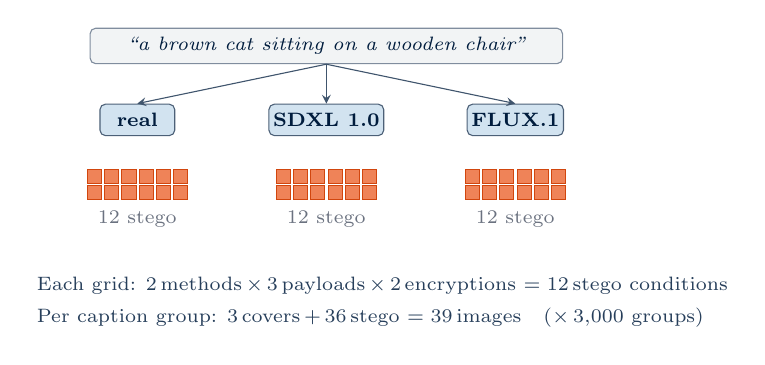
\begin{tikzpicture}[
  capbox/.style={draw=umdark!50, fill=umdark!5, rounded corners=2pt, font=\scriptsize\itshape\color{umdark}, inner sep=2pt, minimum width=6.0cm, minimum height=0.45cm, align=center},
  srcbox/.style={draw=umdark!70, fill=umlight!25, rounded corners=2pt, font=\scriptsize\bfseries\color{umdark}, inner sep=1.5pt, minimum width=0.95cm, minimum height=0.4cm, align=center},
  condcell/.style={draw=umorange!90!black, fill=umorange!70, inner sep=0pt, minimum width=0.18cm, minimum height=0.18cm, line width=0.2pt},
  parrow/.style={->, >=stealth, umdark!75, line width=0.4pt},
]
% Caption at top
\node[capbox] (cap) {``a brown cat sitting on a wooden chair''};

% Three source nodes
\node[srcbox, below=0.50cm of cap, xshift=-2.4cm] (real) {real};
\node[srcbox, below=0.50cm of cap]                (mla)  {SDXL 1.0};
\node[srcbox, below=0.50cm of cap, xshift= 2.4cm] (mlb)  {FLUX.1};

% Arrows from caption
\draw[parrow] (cap.south) -- (real.north);
\draw[parrow] (cap.south) -- (mla.north);
\draw[parrow] (cap.south) -- (mlb.north);

% 12-condition grid under each source: 2 rows x 6 cols
\foreach \xc/\src in {-2.4/real, 0/mla, 2.4/mlb} {
  \foreach \r in {0,1} {
    \foreach \c in {0,1,2,3,4,5} {
      \pgfmathsetmacro{\xx}{\xc - 0.55 + 0.22*\c}
      \pgfmathsetmacro{\yy}{-1.65 - 0.21*\r}
      \node[condcell] at (\xx,\yy) {};
    }
  }
}
% Labels below conditions
\node[font=\scriptsize\color{umgray}] at (-2.4,-2.20) {12 stego};
\node[font=\scriptsize\color{umgray}] at ( 0  ,-2.20) {12 stego};
\node[font=\scriptsize\color{umgray}] at ( 2.4,-2.20) {12 stego};

% Legend explaining grid
\node[font=\scriptsize\color{umdark!85}, align=left, anchor=west] at (-3.8,-3.05) {Each grid: $2$\,methods\,$\times\,3$\,payloads\,$\times\,2$\,encryptions $=12$\,stego conditions};
\node[font=\scriptsize\color{umdark!85}, align=left, anchor=west] at (-3.8,-3.45) {Per caption group: $3$\,covers\,+\,$36$\,stego $=39$\,images\quad($\times\,3{,}000$ groups)};
\end{tikzpicture}
\caption{Caption-matched $3\!\times\!2\!\times\!3\!\times\!2$ factorial design. Each of $N\!=\!3{,}000$ caption groups produces three covers (one per carrier source) under the same caption, then a per-source $2$-method $\times\,3$-payload $\times\,2$-encryption grid of stego variants. Caption-matching holds semantic content constant across sources so that any AUC contrast can only reflect carrier-source statistics, not subject-matter shift.}
\label{fig:factorial}
\end{figure}

\subsection{Embedding Pipeline}
\label{sec:embedding}

\paragraph{Spatial branch (LSB substitution).} Replace the least-significant bit of each pixel in row-major order with payload bits, $k\!=\!1$, until the target fill fraction is reached. Storage is lossless PNG. The mechanism is illustrated in Figure~\ref{fig:lsbdct}~(left).

\paragraph{Frequency branch (JSteg-style DCT-LSB).} Flip the LSB of each non-zero quantised AC DCT coefficient in row-major block order. We skip DC and $|c|\!=\!1$ coefficients to avoid the Westfeld-pair instability they create. Re-entropy-coding uses the same Q=95 table without re-quantisation. The mechanism is illustrated in Figure~\ref{fig:lsbdct}~(right).

\paragraph{Payload levels.} The proposal's original fill rates of $\{0.25,\,0.50,\,0.75\}$ caused near-saturation on the strongest detectors (AUC$\,>\,0.99$), erasing the carrier-source signal. We revised them to $\{0.05,\,0.15,\,0.30\}$~bpp, which is also closer to operationally realistic embedding rates. Both branches use $k\!=\!1$ throughout.

\paragraph{Encryption.} Payloads are tested in two conditions, \emph{plain} (raw bitstream) and \emph{AES-256-CBC} (random IV per message; key fixed per run), in both branches. The encrypted condition tests whether detectors are reacting to plaintext structure rather than to embedding distortion.

\paragraph{Payload distribution: uniform random by construction.} \emph{Plain} in our setting means a uniform random bytestream produced by a seeded RNG (\texttt{payload\_seed=42}), not human-readable text. This is the standard steganalysis-benchmark choice~\cite{boroumand2019srnet,holub2015dctr} and reflects the realistic threat model: any sophisticated attacker encrypts before embedding, and a secure cipher's output is by definition computationally indistinguishable from uniform random. Our \emph{plain} and \emph{AES-256-CBC} conditions therefore both produce maximum-entropy payloads at the bit level, and the choice between them tests a methodological assumption rather than a substantive embedding-distortion property. The encryption-invariance result of RQ5 (Section~\ref{sec:rq5}) empirically validates this assumption -- if it had failed, the use of random-byte payloads as a proxy for encrypted real plaintext would itself have been suspect.

\begin{figure*}[t]
\centering
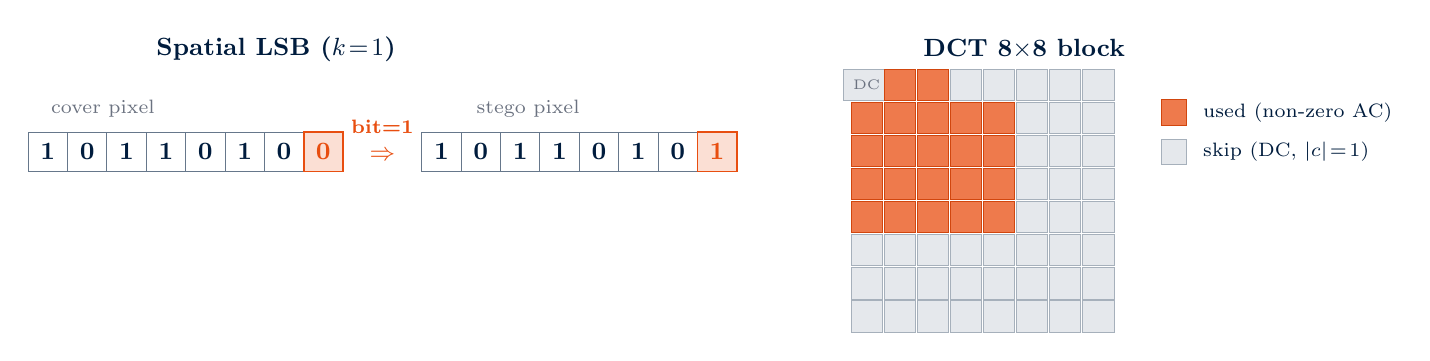
\begin{tikzpicture}[node distance=0.4cm,
  bitcell/.style={draw=umdark!60, minimum width=0.50cm, minimum height=0.50cm, font=\small\bfseries\color{umdark}, line width=0.3pt},
  bitlsb/.style={draw=umorange, fill=umorange!18, minimum width=0.50cm, minimum height=0.50cm, font=\small\bfseries\color{umorange}, line width=0.6pt},
  dctused/.style={draw=umorange!90!black, fill=umorange!75, minimum width=0.40cm, minimum height=0.40cm, line width=0.3pt},
  dctskip/.style={draw=umdark!35, fill=umdark!10, minimum width=0.40cm, minimum height=0.40cm, line width=0.3pt, font=\tiny\color{umgray}},
]
% Left panel: LSB illustration. Origin near x=-7.
\node[font=\small\bfseries\color{umdark}] at (-4.0, 1.3) {Spatial LSB ($k\!=\!1$)};
\node[font=\scriptsize\color{umgray}] at (-6.2, 0.55) {cover pixel};
\foreach \i/\b in {0/1,1/0,2/1,3/1,4/0,5/1,6/0} {
  \pgfmathsetmacro{\xx}{-6.9+0.50*\i}
  \node[bitcell] at (\xx,0) {\b};
}
\node[bitlsb] at (-3.40,0) {0};
\node[font=\scriptsize\bfseries\color{umorange}] at (-2.65,0.32) {bit=1};
\node[font=\small\bfseries\color{umorange}] at (-2.65,-0.05) {$\Rightarrow$};
\node[font=\scriptsize\color{umgray}] at (-0.80, 0.55) {stego pixel};
\foreach \i/\b in {0/1,1/0,2/1,3/1,4/0,5/1,6/0} {
  \pgfmathsetmacro{\xx}{-1.90+0.50*\i}
  \node[bitcell] at (\xx,0) {\b};
}
\node[bitlsb] at (1.60,0) {1};

% Right panel: DCT 8x8 grid (origin around x=4)
\node[font=\small\bfseries\color{umdark}] at (5.5, 1.3) {DCT 8$\times$8 block};
\foreach \r in {0,...,7} {
  \foreach \c in {0,...,7} {
    \pgfmathsetmacro{\xx}{3.5+0.42*\c}
    \pgfmathsetmacro{\yy}{0.85-0.42*\r}
    \ifnum\r=0
      \ifnum\c=0
        \node[dctskip] at (\xx,\yy) {DC};
      \else
        \ifnum\c<3 \node[dctused] at (\xx,\yy) {}; \else \node[dctskip] at (\xx,\yy) {}; \fi
      \fi
    \else
      \ifnum\r>4 \node[dctskip] at (\xx,\yy) {}; \else
        \ifnum\c>4 \node[dctskip] at (\xx,\yy) {}; \else
          \node[dctused] at (\xx,\yy) {};
        \fi
      \fi
    \fi
  }
}
% Legend to the right of the block, well inside textwidth
\node[dctused, minimum size=0.32cm] at (7.4,0.5) {};
\node[font=\scriptsize\color{umdark}, right=2pt] at (7.58,0.5) {used (non-zero AC)};
\node[dctskip, minimum size=0.32cm] at (7.4,0.0) {};
\node[font=\scriptsize\color{umdark}, right=2pt] at (7.58,0.0) {skip (DC, $|c|\!=\!1$)};
\end{tikzpicture}
\vspace{-2mm}
\caption{Embedding mechanisms. \textbf{Left:} spatial LSB replacement, one cover bit overwritten per pixel in row-major order. \textbf{Right:} DCT-LSB on JPEG Q=95, where the LSB of each non-zero AC coefficient is flipped; DC and $|c|\!=\!1$ are skipped.}
\label{fig:lsbdct}
\end{figure*}

\subsection{Detectors}
\label{sec:detectors}

Six training-free detectors are scored on every (cover, stego) pair:
\begin{itemize}
\item \textbf{Spatial branch (PNG):} RS Analysis~\cite{fridrich2001lsb}, Westfeld $\chi^2$ on pixel-value pairs ($\chi^2$-spatial)~\cite{westfeld1999chi}, Sample Pairs~\cite{dumitrescu2003sp}.
\item \textbf{Frequency branch (JPEG):} Westfeld $\chi^2$ on quantised AC DCT coefficients ($\chi^2$-DCT)~\cite{westfeld1999chi}, our \textbf{tile-local $\chi^2$-DCT variant} ($\chi^2$-DCTt, Section~\ref{sec:tiled}), and Fridrich's calibration $\chi^2$~\cite{fridrich2003calib}.
\end{itemize}

\paragraph{Underflow-free scoring.} All chi-square detectors are rank-monotonic with the Westfeld~1999 p-value but use the \emph{underflow-free} $-\chi^2_\text{stat}/(df\!-\!1)$ transformation, because chi-square p-values vanish under float64 representation on large textured images. Listing~\ref{lst:chispatial} shows the spatial-$\chi^2$ implementation.

\begin{lstlisting}[label={lst:chispatial},caption={Spatial $\chi^2$ (Westfeld~1999) on a grayscale image, with the underflow-free score transformation. The classical p-value is replaced by $-\chi^2/df$ which is rank-monotonic with the p-value on non-degenerate inputs but does not collapse to zero on large textured images.}]
def chi_square_spatial_score(image: Image.Image) -> float:
    pixels = np.array(image.convert("L")).flatten()
    counts = np.bincount(pixels, minlength=256)
    chi_stat, df = 0.0, 0
    for k in range(128):
        n_2k, n_2k1 = counts[2*k], counts[2*k+1]
        expected = (n_2k + n_2k1) / 2.0
        if expected > 0:
            chi_stat += ((n_2k - expected) ** 2) / expected
            df += 1
    return 0.0 if df <= 1 else -float(chi_stat) / (df - 1)
\end{lstlisting}

\subsection{Learned Detectors for Cross-Validation (SRNet, DCTR)}
\label{sec:learned-detectors}

Two state-of-the-art learned detectors are added as a methodologically orthogonal cross-validation of the pre-registered protocol, one per embedding branch. They are trained on a corpus disjoint from the test set by caption~ID; the same DeLong + Bonferroni--Holm + $\delta_\text{min}$ machinery used for the classical detectors is applied to a separate 6-stratum family of learned-detector contrasts (Section~\ref{sec:learnedxval}).

\paragraph{SRNet (spatial branch).} The 12-block residual network of Boroumand~et~al.~\cite{boroumand2019srnet} (Type~1$\times$2, Type~2$\times$5, Type~3$\times$4, Type~4$\times$1) with channel widths $\{64,16,16{\times}5,16,64,128,256,512\}$ matching the published Figure~2 and a $512{\rightarrow}2$ fully-connected head. We faithfully include the Type~4 residual skip (some open-source ports omit it). Our implementation totals 4.93M trainable parameters; the paper claims 467k but Figure~2 composes to $\sim$4.9M and other open-source ports also land in the $2$--$5$M range. No TLU (paper-correct); BatchNorm throughout; Adamax (lr $10^{-3}$, paper-faithful) with reduce-on-plateau on validation AUC, gradient $L_2$ clip at 1.0, and the D4 dihedral augmentation paired sampler.

\paragraph{DCTR (frequency branch).} The 1{,}280-dimensional canonical DCTR feature set (64 DCT modes $\times$ 4 cosets $\times$ 5 truncated-absolute-value bins, T=4)~\cite{holub2015dctr}, computed via undecimated DCT with mode-specific quantization from the standard JPEG luminance table at Q=95. Per-image extraction is $\sim$80~ms on one core. The classifier is a Fisher-LDA ensemble in the Kodovsk\'{y}-Fridrich style~\cite{fridrich2012srm}, implemented as scikit-learn's \texttt{BaggingClassifier(LinearDiscriminantAnalysis, n\_estimators=100, max\_features=0.1, bootstrap=True)} on standardised features.

\paragraph{Per-cell training.} Following steganalysis-literature standard we train one model per (method, payload) cell: three SRNet checkpoints (LSB / \{low, medium, high\}) and three DCTR ensembles (DCT / \{low, medium, high\}), six trained detectors total. Each detector scores only its own embedding branch; the LSB cells are fanned across rs / sample\_pairs / $\chi^2$-spatial / SRNet, and the DCT cells across $\chi^2$-DCT / $\chi^2$-DCT-tiled / calibration-$\chi^2$ / DCTR -- so within each branch we obtain a clean four-way detector comparison on identical test cells.

\paragraph{Training data and leakage guard.} The learned detectors are trained on a \emph{separate} 3{,}000-group caption-matched corpus (Section~\ref{sec:learnedxval}); the training caption pool excludes all 3{,}000 caption~IDs that appear in the test run. The training-set manifest is hashed (SHA-256, leading 16 hex digits) and embedded in every saved checkpoint; the inference scripts refuse to apply a checkpoint to any run whose manifest hash matches the training hash, programmatically preventing train/test leakage. Encryption is handled symmetrically with the classical analysis: at training time each cover is paired with a randomly chosen encryption variant; at inference time each cover is scored once and the score is fanned out to one row per encryption variant (cover bytes are identical regardless of encryption, so one score per cover is correct).

\paragraph{V2a real-only-training ablation.} The primary learned-detector training (``V1'') uses the same 3-source carrier balance (real + SDXL + FLUX, 1:1:1) as the test set, so SRNet sees all carrier types during training. Any source-invariance observed at inference time could then be either an architectural property of the CNN or an artefact of balanced training exposure. A second training run (``V2a'') trains the same six checkpoints on a \emph{real-only} corpus of disjoint Flickr30k captions, holding sample count constant; the resulting source-AUC pattern at test time disentangles the two interpretations (\S\ref{sec:v2a}).

\paragraph{Reporting protocol.} The learned-detector contrasts use the same DeLong test, Bonferroni--Holm correction, and $\delta_\text{min}$ thresholds as the classical detectors, with their own 6 (method$\times$payload) strata per RQ. The Bonferroni--Holm family is computed \emph{separately} for the classical and learned detectors; the pre-registered classical-detector correction in Table~\ref{tab:verdicts} is not silently rewritten.

\subsection{Statistical Protocol}
\label{sec:stats}

The unit of analysis is a \emph{stratum}: a (detector $\times$ embedding method $\times$ payload level) cell. For RQ1 and RQ2 we have $6\!\times\!3\!=\!18$ strata each. Within each stratum we compute the area under the ROC curve (AUC) for both carrier groups and the \textbf{paired AUC difference} via the \textbf{DeLong test}~\cite{delong1988}, which exploits the fact that the same covers are scored in both groups; the pairing eliminates between-image variance and substantially increases statistical power.

The 18 stratum-level p-values are corrected with \textbf{Bonferroni--Holm} at $\alpha\!=\!0.05$ for the confirmatory RQs (RQ1, RQ2); RQ3 and RQ4 use 95\% confidence intervals; RQ5 uses an equivalence test against a $\pm0.025$ AUC margin. A stratum is declared \textbf{practically significant} only if \emph{both} $p_\text{Holm}\!\leq\!0.05$ \emph{and} $|\Delta_\text{AUC}|\!\geq\!\delta_\text{min}$. The pooled $\Delta_\text{AUC}$ across strata is inverse-variance-weighted.

\paragraph{Two thresholds on $\delta_\text{min}$.} The proposal pre-registered $\delta_\text{min}\!=\!0.05$, calibrated to the Hanley--McNeil minimum-detectable effect at $\alpha\!=\!0.05$, $80\%$ power and $N\!=\!1{,}000$. At the confirmatory $N\!=\!3{,}000$ the same power calculation gives a minimum-detectable effect of $\approx\!0.029$; the sample-size-matched threshold is therefore $\delta_\text{min}\!=\!0.025$. We report verdicts at \emph{both} thresholds: $\delta_\text{min}\!=\!0.05$ remains the \textbf{primary} (pre-registered) outcome, and $\delta_\text{min}\!=\!0.025$ is reported as a \textbf{supplementary} sensitivity analysis. This avoids moving the goalposts after the fact while transparently exposing what the data says under the threshold the larger sample's power actually supports.

The verdict assignment follows the decision rule in Table~\ref{tab:verdictrule}.

\begin{table}[!htbp]
\centering\small
\caption{Verdict assignment rule for confirmatory RQs.}
\label{tab:verdictrule}
\setlength{\tabcolsep}{6pt}\renewcommand{\arraystretch}{1.1}
\begin{tabular}{@{}lll@{}}
\toprule
\textbf{Significant strata} & \textbf{Practical strata} & \textbf{Verdict} \\
\midrule
0 / family            & --             & \emph{not supported} \\
$\geq\!1$, mixed sign & $\geq\!1$      & \textbf{mixed}       \\
$\geq\!1$, same sign  & $\geq\!1$      & \textbf{supported}   \\
$\geq\!1$             & 0              & \emph{trivial}       \\
\bottomrule
\end{tabular}
\end{table}

\subsection{Score-level Sanity Checks (t-test and Wilcoxon)}
\label{sec:scorelevel}
The DeLong test operates at the \emph{ROC AUC} level: it asks whether the detector's \emph{ranking ability} differs between two carrier groups. As a complementary sanity check we also run paired \textbf{t-tests} and \textbf{Wilcoxon signed-rank tests} on the \emph{raw detector scores} for the four pre-registered comparisons (real vs.\ SDXL, real vs.\ FLUX, SDXL vs.\ FLUX, plain vs.\ AES-256-CBC), per detector. These score-level tests detect whether the score \emph{distributions} differ even when the ranking-based AUC contrast is null, and report effect sizes (Cohen's $d$ for t-test, $r$ for Wilcoxon). They are reported as supplementary diagnostics in Appendix~\ref{app:t-tests}; DeLong remains the test of record for the verdicts. A score-level shift without an AUC change indicates that detectors recognise the carrier source distribution but do not gain ranking power from the difference -- exactly the pattern we observe for RQ5 below.

\subsection{Supplementary Partial-AUC Analysis}
\label{sec:pauc}

Full AUC integrates the ROC curve over all false-positive rates, including regions a real steganalyst would never deploy. As a supplementary analysis we therefore re-run RQ1 and RQ2 on the \textbf{McClish-normalised partial AUC} at FPR\,$\leq\!0.10$~\cite{mcclish1989}. Bootstrap standard errors (500 resamples per stratum) replace the DeLong estimator (which has no exact closed-form analogue at low-FPR pAUC), and Holm correction and the practical-significance gate are applied identically to the full-AUC analysis. The choice of FPR cap follows the McClish standard, matches steganalysis screening practice, and fits the shape of our ROC curves.

\subsection{Sample Size and Power}

At $N\!=\!1{,}000$ groups per source, the Hanley--McNeil power calculation shows the smallest detectable AUC difference at $\alpha\!=\!0.05$ and $80\%$ power is below the $\delta_\text{min}\!=\!0.05$ threshold for every stratum in RQ1, RQ2 and RQ5. The $N\!=\!3{,}000$ confirmatory run reported here tightens every CI by a factor of $\sqrt{3}\!\approx\!1.73$ and serves as an independent replication of the pre-registered $N\!=\!1{,}000$ findings.

% ============================================================
\section{Experiments}
\label{sec:experiments}
% ============================================================

\subsection{Run Configuration}
The full factorial was executed once at $N\!=\!1{,}000$ groups (pre-registered) and again at $N\!=\!3{,}000$ groups (confirmatory). The pipeline (Figure~\ref{fig:pipeline}) is implemented in Python, runs from a frozen \texttt{config.json}, and is reproducible from seed. The active configuration of the $N\!=\!3{,}000$ run is listed in Appendix~\ref{app:config}.

\begin{figure}[t]
\centering
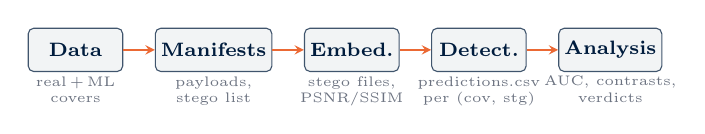
\begin{tikzpicture}[
  pstage/.style={draw=umdark!75, fill=umdark!5, rounded corners=2pt, font=\scriptsize\bfseries\color{umdark}, inner sep=2pt, minimum width=1.20cm, minimum height=0.55cm, align=center},
  pout/.style={font=\tiny\color{umgray}, align=center, inner sep=0pt},
  parrow/.style={->, >=stealth, umorange!85, line width=0.5pt},
]
\node[pstage] (data) {Data};
\node[pstage, right=0.40cm of data] (man)  {Manifests};
\node[pstage, right=0.40cm of man]  (emb)  {Embed.};
\node[pstage, right=0.40cm of emb]  (det)  {Detect.};
\node[pstage, right=0.40cm of det]  (agg)  {Analysis};
\draw[parrow] (data) -- (man);
\draw[parrow] (man)  -- (emb);
\draw[parrow] (emb)  -- (det);
\draw[parrow] (det)  -- (agg);
\node[pout, below=0.05cm of data] {real\,+\,ML\\ covers};
\node[pout, below=0.05cm of man]  {payloads,\\ stego list};
\node[pout, below=0.05cm of emb]  {stego files,\\ PSNR/SSIM};
\node[pout, below=0.05cm of det]  {predictions.csv\\ per (cov, stg)};
\node[pout, below=0.05cm of agg]  {AUC, contrasts,\\ verdicts};
\end{tikzpicture}
\caption{Five-stage pipeline. Each stage reads files written by the previous stage; manifests freeze the experimental design before any compute runs, and the analysis stage derives every contrast in this paper from a single \texttt{predictions.csv}.}
\label{fig:pipeline}
\end{figure}

\paragraph{Learned-detector training run (V1).} A separate 3{,}000-group training run was executed on a rented Vast.ai cloud instance (RTX~5880~Ada) to produce the SRNet and DCTR checkpoints (Section~\ref{sec:learned-detectors}). It uses the same factorial design as the test run (real + ML-A + ML-B carriers, LSB + DCT methods, three payload levels, two encryption modes) but draws caption~IDs from a pool that programmatically excludes every caption~ID in the test run's manifest. Per-checkpoint sample count is $n_\text{train}\!=\!18{,}900$ and $n_\text{val}\!=\!5{,}292$ (1 cover + 2 stego variants per cover-group at 80/20 group-level split). Training-run wall-clock was approximately 8~h end-to-end for $\sim\$$8; the resulting six checkpoints (3 SRNet + 3 DCTR), per-cell training logs, and the SHA-256 manifest hash of the training data are all included in the supplementary deliverables bundle.

\paragraph{Learned-detector ablation run (V2a).} A second training run with the same sample-count budget but real-only carriers (9{,}000 Flickr30k captions disjoint from both the test run and V1's training-caption set) was executed on the same Vast.ai instance type. V2a uses 100\% Flickr30k because the disjoint-from-test COCO caption pool is below the 1.75$\times$ overshoot the download pipeline needs at $n\!=\!9{,}000$; both Flickr30k and COCO are natural-image datasets and the source-invariance hypothesis under test (Section~\ref{sec:v2a}) is dataset-agnostic. Six additional checkpoints (3 SRNet-v2a + 3 DCTR-v2a) are produced; per-checkpoint sample counts match V1.

\subsection{Artefacts Produced}
The $N\!=\!3{,}000$ test run produced 18{,}000 covers, 108{,}000 stego images, 648{,}000 classical-detector predictions, 19 metrics CSVs, 61 figures, and the per-RQ verdicts in JSON and Markdown. Total wall-clock was approximately 13~h, of which \textasciitilde6~h was cover generation (HF Inference API throughput-bound), \textasciitilde2~h was embedding, \textasciitilde0.5~h was detection, and the remainder was analysis. The analysis-stage cost has since been reduced by an order of magnitude (factor $\sim$560$\times$) by replacing the pure-Python $O(N^2)$ ROC threshold sweep with a numpy sort+cumsum implementation, used throughout the cross-validation analyses of Section~\ref{sec:learnedxval}. Learned-detector inference on the same test corpus adds 108{,}000 prediction rows per detector family ($2\times108{,}000$ for V1, another $2\times108{,}000$ for V2a) in separate CSVs that the cross-validation pipeline reads alongside \texttt{predictions.csv}; the parallel \texttt{learned\_shadow/} and \texttt{learned\_shadow\_v2a/} run directories keep the pre-registered classical-detector outputs frozen.

% ============================================================
\section{Results}
\label{sec:results}
% ============================================================

The headline verdicts are summarised in Table~\ref{tab:verdicts}; the rest of this section walks through each RQ with the supporting figures.

\begin{table*}[t]
\centering\footnotesize
\caption{Verdict summary across the five research questions ($N\!=\!3{,}000$ confirmatory run). Verdicts are reported at \emph{two} practical-significance thresholds: $\delta_\text{min}\!=\!0.05$ is the pre-registered primary; $\delta_\text{min}\!=\!0.025$ is the power-matched supplementary at the actual sample size. Practical-count cells read $n_\text{practical}/n_\text{sig}$ followed by $(+\!,-)$ direction breakdown.}
\label{tab:verdicts}
\setlength{\tabcolsep}{6pt}\renewcommand{\arraystretch}{1.1}
\begin{tabular}{@{}l l c c c c c@{}}
\toprule
& & & \multicolumn{2}{c}{\textbf{$\delta_\text{min}\!=\!0.05$ (primary)}} & \multicolumn{2}{c}{\textbf{$\delta_\text{min}\!=\!0.025$ (supplementary)}} \\
\cmidrule(lr){4-5}\cmidrule(lr){6-7}
\textbf{RQ} & \textbf{Pooled $\Delta$} & \textbf{Holm sig.} & \textbf{Practical} & \textbf{Verdict} & \textbf{Practical} & \textbf{Verdict} \\
\midrule
RQ1 real vs ML        & $-0.0129$ & 16/18 & 4/16 (0,$\,$4$-$)  & mixed     & 11/16 (2,$\,$9$-$) & mixed   \\
RQ2 SDXL vs FLUX      & $+0.0004$ & 7/18  & 0/7                & trivial   & 3/7 (2,$\,$1$-$)   & \textbf{mixed} \\
RQ3 payload $\times$ source & gap shrinks with bpp & ---  & --- & supported & ---                 & supported \\
RQ4 spatial $-$ freq. & $-0.0013$ & 2/3   & 0/2                & trivial   & 1/2 (0,$\,$1$-$)   & mixed   \\
RQ5 plain vs AES      & $\sim\!0$ & 0/54 outside & ---         & supported & ---                 & supported \\
\midrule
\multicolumn{7}{@{}l@{}}{\textit{Supplementary partial AUC at FPR\,$\leq\!0.10$:}} \\
RQ1 pAUC              & $-0.0174$ & 12/18 & 6/12 (0,$\,$6$-$)  & \textbf{supported} & 9/12 (0,$\,$9$-$)  & \textbf{supported} \\
RQ2 pAUC              & $+0.0008$ & 7/18  & 1/7                & mixed     & 4/7 (3,$\,$1$-$)   & mixed   \\
\bottomrule
\end{tabular}
\end{table*}

\subsection{Headline AUC by Carrier Source and Detector}

Figure~\ref{fig:headline} plots the mean AUC of every detector against each of the three carrier sources. The visual pattern is immediate: for five of six detectors the orange/blue bars (ML carriers) are higher than the dark bars (real photographs). Only the third bar group ($\chi^2$-spatial) reverses this ordering, with real $>$ ML by a small but consistent margin.

\begin{figure*}[t]
\centering
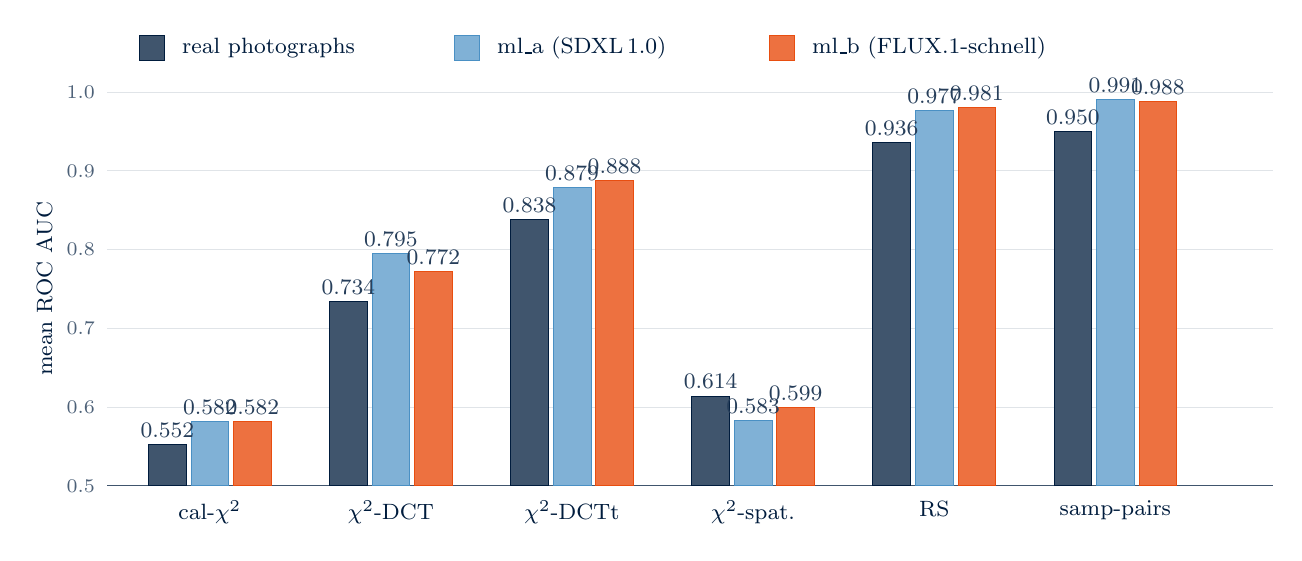
\begin{tikzpicture}[
  bargrey/.style={draw=umdark, fill=umdark!75, line width=0.25pt},
  barblue/.style={draw=umlight, fill=umlight!70, line width=0.25pt},
  baroran/.style={draw=umorange, fill=umorange!80, line width=0.25pt},
]
% y-axis (AUC 0.5..1.0 mapped to 0..5 cm)
\foreach \v in {0.5,0.6,0.7,0.8,0.9,1.0} {
  \pgfmathsetmacro{\y}{(\v - 0.5) * 10}
  \draw[umdark!12, line width=0.3pt] (0,\y) -- (14.8,\y);
  \node[font=\scriptsize\color{umdark!70}, left=1pt] at (0,\y) {\v};
}
\draw[umdark!75, line width=0.5pt] (0,0) -- (14.8,0);
\node[font=\footnotesize\color{umdark}, rotate=90] at (-0.8,2.5) {mean ROC AUC};

\def\bw{0.48}
\def\bg{0.06}
\foreach \i/\name/\real/\mla/\mlb in {%
  0/{cal-$\chi^2$}/0.552/0.582/0.582,
  1/{$\chi^2$-DCT}/0.734/0.795/0.772,
  2/{$\chi^2$-DCTt}/0.838/0.879/0.888,
  3/{$\chi^2$-spat.}/0.614/0.583/0.599,
  4/{RS}/0.936/0.977/0.981,
  5/{samp-pairs}/0.950/0.991/0.988%
} {
  \pgfmathsetmacro{\xc}{1.3 + \i*2.30}
  \pgfmathsetmacro{\xa}{\xc - 1.5*\bw - \bg}
  \pgfmathsetmacro{\xb}{\xc - 0.5*\bw}
  \pgfmathsetmacro{\xcc}{\xc + 0.5*\bw + \bg}
  \pgfmathsetmacro{\hreal}{(\real - 0.5) * 10}
  \pgfmathsetmacro{\hmla}{(\mla - 0.5) * 10}
  \pgfmathsetmacro{\hmlb}{(\mlb - 0.5) * 10}
  \draw[bargrey] (\xa,0)  rectangle (\xa+\bw,\hreal);
  \draw[barblue] (\xb,0)  rectangle (\xb+\bw,\hmla);
  \draw[baroran] (\xcc,0) rectangle (\xcc+\bw,\hmlb);
  \node[font=\footnotesize\color{umdark!85}, above=-1pt] at (\xa+\bw/2, \hreal) {\real};
  \node[font=\footnotesize\color{umdark!85}, above=-1pt] at (\xb+\bw/2, \hmla)  {\mla};
  \node[font=\footnotesize\color{umdark!85}, above=-1pt] at (\xcc+\bw/2,\hmlb) {\mlb};
  \node[font=\footnotesize\color{umdark}, below=2pt] at (\xc,0) {\name};
}
% Legend top-left
\begin{scope}[shift={(0.4, 5.4)}]
  \draw[bargrey] (0,0) rectangle (0.32,0.32); \node[font=\footnotesize\color{umdark}, right=3pt] at (0.32,0.16) {real photographs};
  \draw[barblue] (4.0,0) rectangle (4.32,0.32); \node[font=\footnotesize\color{umdark}, right=3pt] at (4.32,0.16) {ml\_a (SDXL\,1.0)};
  \draw[baroran] (8.0,0) rectangle (8.32,0.32); \node[font=\footnotesize\color{umdark}, right=3pt] at (8.32,0.16) {ml\_b (FLUX.1-schnell)};
\end{scope}
\end{tikzpicture}
\caption{Mean ROC~AUC per detector and carrier source, pooled across payload, encryption and method ($N\!=\!3{,}000$). For five of six detectors the ML bars exceed the real bar (all $\Delta_\text{AUC}\!<\!0$); only $\chi^2$-spatial reverses the ordering (real $>$ ML). Detector ordering left-to-right follows ascending pooled AUC.}
\label{fig:headline}
\end{figure*}

\subsection{RQ1 -- Real vs.\ Pooled ML Carriers}
\label{sec:rq1}

The pooled $\Delta_\text{AUC}\!=\!-0.0129$ (95\%~CI $[-0.0137,-0.0121]$) is small but tightly constrained, with \textbf{16/18 strata} Holm-significant. At the pre-registered $\delta_\text{min}\!=\!0.05$ threshold, \textbf{4 of those 16} strata clear the practical-significance gate, all on the \emph{ML-easier} side: RS/LSB/low ($\Delta\!=\!-0.090$), sample-pairs/LSB/low ($-0.089$), $\chi^2$-DCT-tiled/DCT/low ($-0.060$) and $\chi^2$-DCT/DCT/medium ($-0.051$). Three independent detector families therefore agree on the direction at low-to-medium payload. The primary verdict is \textbf{mixed}: a direction-consistent ML-easier signal at the practical-significance gate but most strata sit inside the trivial band.

At the supplementary $\delta_\text{min}\!=\!0.025$ threshold (Section~\ref{sec:stats}), the practical count rises to \textbf{11/16}: nine ML-easier strata across five detector families (cal-$\chi^2$/dct/high, $\chi^2$-DCT/dct at all three payloads, $\chi^2$-DCT-tiled/dct/low and /medium, RS/LSB/low and /medium, sample-pairs/LSB/low) plus two $\chi^2$-spatial strata on the real-easier side (medium $\Delta\!=\!+0.027$, high $\Delta\!=\!+0.034$). The verdict remains \textbf{mixed}; the carrier-source effect is robust to threshold choice in direction, and at the larger threshold the evidence base is roughly $2.75\!\times\!$ deeper.

The single dissenter is $\chi^2$-spatial: real photographs are \emph{easier} to attack than ML carriers at medium ($\Delta\!=\!+0.027$) and high payload ($+0.034$), both Holm-significant and both clearing the $\delta_\text{min}\!=\!0.025$ threshold; low payload sits inside the trivial band even at 0.025. We return to this reversal in Section~\ref{sec:chi2spatial}.

Figure~\ref{fig:rq1strip} renders the 18 strata as a strip plot, one row per detector. Each detector's three payload-level $\Delta_\text{AUC}$ are connected to expose payload trends. The four dots outside the practical band (RS/LSB/low, sample-pairs/LSB/low, $\chi^2$-DCT-tiled/DCT/low, $\chi^2$-DCT/DCT/medium) belong to three independent detector families, and the three $\chi^2$-spatial dots are the lone real-easier outliers. Table~\ref{tab:rq1meta} aggregates the strip plot per detector via inverse-variance pooling, making the direction-of-effect at the detector-family level easier to read off.

\begin{figure}[t]
\centering
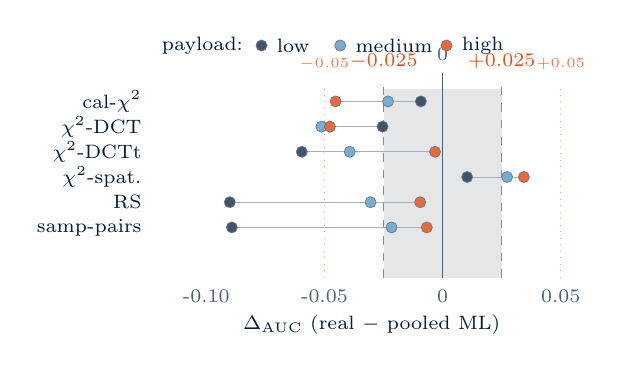
\begin{tikzpicture}[
  detrow/.style={font=\scriptsize\color{umdark}},
  dotlow/.style={circle, draw=umdark!60, fill=umdark!75,    inner sep=0pt, minimum size=4pt, line width=0.25pt},
  dotmed/.style={circle, draw=umdark!60, fill=umlight!75,   inner sep=0pt, minimum size=4pt, line width=0.25pt},
  dothigh/.style={circle, draw=umdark!60, fill=umorange!85, inner sep=0pt, minimum size=4pt, line width=0.25pt},
]
% x mapping: Δ in [-0.12, +0.06] -> [0, 5.4] cm (multiplier 30)
% ± 0.025 lives at x = 2.85 / 4.35; ± 0.05 lives at x = 2.1 / 5.1
% Grey band = supplementary threshold |Δ|<0.025 (the tighter/primary visual band);
% dotted lines at ±0.05 = pre-registered threshold.
\fill[umgray!18] (2.85,-2.3) rectangle (4.35,0.10);
\draw[umdark!70, line width=0.4pt] (3.6,-2.3) -- (3.6,0.30);
\node[font=\scriptsize\color{umdark!70}, above=1pt] at (3.6,0.30) {0};
\draw[umorange!85, line width=0.4pt, dashed] (2.85,-2.3) -- (2.85,0.20);
\draw[umorange!85, line width=0.4pt, dashed] (4.35,-2.3) -- (4.35,0.20);
\node[font=\scriptsize\color{umorange}, above=1pt] at (2.85,0.20) {$-0.025$};
\node[font=\scriptsize\color{umorange}, above=1pt] at (4.35,0.20) {$+0.025$};
\draw[umorange!55, line width=0.35pt, dotted] (2.1,-2.3) -- (2.1,0.10);
\draw[umorange!55, line width=0.35pt, dotted] (5.1,-2.3) -- (5.1,0.10);
\node[font=\tiny\color{umorange!75}] at (2.1,0.42) {$-0.05$};
\node[font=\tiny\color{umorange!75}] at (5.1,0.42) {$+0.05$};
\foreach \v in {-0.10,-0.05,0,0.05} {
  \pgfmathsetmacro{\x}{(\v + 0.12) * 30}
  \node[font=\scriptsize\color{umdark!70}, below=1pt] at (\x,-2.3) {\v};
}
\node[font=\scriptsize\color{umdark}, below=10pt] at (2.7,-2.3) {$\Delta_\text{AUC}$ (real $-$ pooled ML)};

\foreach \i/\labl/\dl/\dm/\dh in {%
  0/{cal-$\chi^2$}/-0.0092/-0.0231/-0.0453,
  1/{$\chi^2$-DCT}/-0.0254/-0.0513/-0.0477,
  2/{$\chi^2$-DCTt}/-0.0596/-0.0393/-0.0032,
  3/{$\chi^2$-spat.}/0.0104/0.0273/0.0344,
  4/{RS}/-0.0901/-0.0305/-0.0095,
  5/{samp-pairs}/-0.0892/-0.0216/-0.0067%
} {
  \pgfmathsetmacro{\y}{-\i*0.32 - 0.06}
  \node[detrow, anchor=east] at (-0.10,\y) {\labl};
  \pgfmathsetmacro{\xa}{(\dl + 0.12) * 30}
  \pgfmathsetmacro{\xb}{(\dm + 0.12) * 30}
  \pgfmathsetmacro{\xcc}{(\dh + 0.12) * 30}
  \draw[umdark!35, line width=0.35pt] (\xa,\y) -- (\xcc,\y);
  \node[dotlow]  at (\xa,\y) {};
  \node[dotmed]  at (\xb,\y) {};
  \node[dothigh] at (\xcc,\y) {};
}
% legend (top of plot)
\node[font=\scriptsize\color{umdark}] at (0.55,0.65) {payload:};
\node[dotlow]  at (1.30,0.65) {};
\node[font=\scriptsize\color{umdark}, right=2pt] at (1.30,0.65) {low};
\node[dotmed]  at (2.30,0.65) {};
\node[font=\scriptsize\color{umdark}, right=2pt] at (2.30,0.65) {medium};
\node[dothigh] at (3.65,0.65) {};
\node[font=\scriptsize\color{umdark}, right=2pt] at (3.65,0.65) {high};
\end{tikzpicture}
\caption{RQ1 -- paired DeLong $\Delta_\text{AUC}$ per stratum (real $-$ pooled ML), $N\!=\!3{,}000$. Each detector row spans its three payload strata. The grey band marks the supplementary trivial zone $|\Delta|\!<\!0.025$ (dashed orange boundaries, power-matched to $N\!=\!3{,}000$); the dotted orange lines at $\pm 0.05$ mark the pre-registered threshold. Eleven dots clear the supplementary gate and four clear the pre-registered one (RS/low, sample-pairs/low, $\chi^2$-DCT-tiled/low, $\chi^2$-DCT/medium), all on the ML-easier side; $\chi^2$-spatial's medium and high strata clear the supplementary gate on the opposite side.}
\label{fig:rq1strip}
\end{figure}

\begin{table}[t]
\centering\small
\caption{RQ1 -- per-detector inverse-variance pooled $\Delta_\text{AUC}$ across the three payload strata ($k\!=\!3$). All meta values negative except $\chi^2$-spatial.}
\label{tab:rq1meta}
\setlength{\tabcolsep}{5pt}\renewcommand{\arraystretch}{1.1}
\begin{tabular}{@{}l r l@{}}
\toprule
\textbf{Detector} & \textbf{Pooled $\Delta$} & \textbf{95\% CI} \\
\midrule
calibration $\chi^2$    & $-0.026$ & $[-0.033, -0.019]$ \\
$\chi^2$-DCT            & $-0.045$ & $[-0.050, -0.040]$ \\
$\chi^2$-DCT-tiled      & $-0.006$ & $[-0.008, -0.005]$ \\
$\chi^2$-spatial        & $+0.025$ & $[+0.018, +0.032]$ \\
RS                      & $-0.015$ & $[-0.016, -0.014]$ \\
sample-pairs            & $-0.014$ & $[-0.015, -0.012]$ \\
\midrule
\textbf{All strata}     & $\boldsymbol{-0.013}$ & $\boldsymbol{[-0.014, -0.012]}$ \\
\bottomrule
\end{tabular}
\end{table}

\subsection{RQ2 -- SDXL vs.\ FLUX within ML}

The pooled $\Delta_\text{AUC}\!=\!+0.0004$ is essentially zero. 7/18 strata are Holm-significant under the larger sample size, and the strata are mixed in direction (four favour SDXL, three FLUX). At the pre-registered $\delta_\text{min}\!=\!0.05$, \textbf{none of the seven Holm-significant strata clear the practical-significance gate} -- the primary verdict is \textbf{trivial} (Figure~\ref{fig:rq2}). At the supplementary $\delta_\text{min}\!=\!0.025$, three strata clear the tighter gate ($\chi^2$-DCT/dct/medium $+0.031$, $\chi^2$-DCT/dct/high $+0.025$, $\chi^2$-spatial/LSB/high $-0.029$), so the verdict shifts to \textbf{mixed}; however, no detector family is unanimous across payloads, so the directional-consistency criterion that would support a "generator effect" claim still fails.

\begin{figure}[t]
\centering
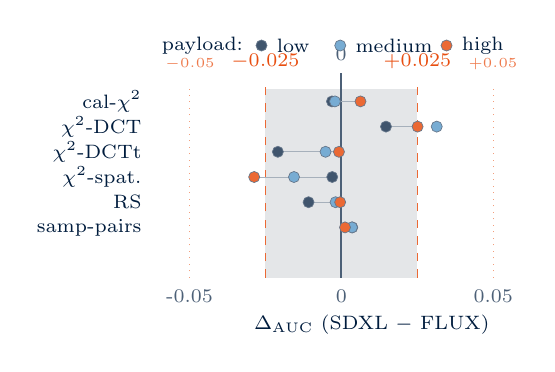
\begin{tikzpicture}[
  detrow/.style={font=\scriptsize\color{umdark}},
  dotlow/.style={circle, draw=umdark!60, fill=umdark!75,    inner sep=0pt, minimum size=4pt, line width=0.25pt},
  dotmed/.style={circle, draw=umdark!60, fill=umlight!75,   inner sep=0pt, minimum size=4pt, line width=0.25pt},
  dothigh/.style={circle, draw=umdark!60, fill=umorange!85, inner sep=0pt, minimum size=4pt, line width=0.25pt},
]
% RQ2 scale: Δ in [-0.06, +0.08] -> [0, 5.4] cm.
% ± 0.025 lives at x = 1.35 / 3.28; ± 0.05 lives at x = 0.39 / 4.24
\fill[umgray!18] (1.35,-2.3) rectangle (3.28,0.10);
\draw[umdark!70, line width=0.4pt] (2.31,-2.3) -- (2.31,0.30);
\node[font=\scriptsize\color{umdark!70}, above=1pt] at (2.31,0.30) {0};
\draw[umorange!85, line width=0.4pt, dashed] (1.35,-2.3) -- (1.35,0.20);
\draw[umorange!85, line width=0.4pt, dashed] (3.28,-2.3) -- (3.28,0.20);
\node[font=\scriptsize\color{umorange}, above=1pt] at (1.35,0.20) {$-0.025$};
\node[font=\scriptsize\color{umorange}, above=1pt] at (3.28,0.20) {$+0.025$};
\draw[umorange!55, line width=0.35pt, dotted] (0.39,-2.3) -- (0.39,0.10);
\draw[umorange!55, line width=0.35pt, dotted] (4.24,-2.3) -- (4.24,0.10);
\node[font=\tiny\color{umorange!75}] at (0.39,0.42) {$-0.05$};
\node[font=\tiny\color{umorange!75}] at (4.24,0.42) {$+0.05$};
\foreach \v in {-0.05,0,0.05} {
  \pgfmathsetmacro{\x}{(\v + 0.06) / 0.14 * 5.4}
  \node[font=\scriptsize\color{umdark!70}, below=1pt] at (\x,-2.3) {\v};
}
\node[font=\scriptsize\color{umdark}, below=10pt] at (2.7,-2.3) {$\Delta_\text{AUC}$ (SDXL $-$ FLUX)};

\foreach \i/\labl/\dl/\dm/\dh in {%
  0/{cal-$\chi^2$}/-0.0031/-0.0021/0.0063,
  1/{$\chi^2$-DCT}/0.0147/0.0314/0.0251,
  2/{$\chi^2$-DCTt}/-0.0209/-0.0052/-0.0008,
  3/{$\chi^2$-spat.}/-0.0030/-0.0156/-0.0287,
  4/{RS}/-0.0108/-0.0019/-0.0004,
  5/{samp-pairs}/0.0036/0.0035/0.0012%
} {
  \pgfmathsetmacro{\y}{-\i*0.32 - 0.06}
  \node[detrow, anchor=east] at (-0.10,\y) {\labl};
  \pgfmathsetmacro{\xa}{(\dl + 0.06) / 0.14 * 5.4}
  \pgfmathsetmacro{\xb}{(\dm + 0.06) / 0.14 * 5.4}
  \pgfmathsetmacro{\xcc}{(\dh + 0.06) / 0.14 * 5.4}
  \draw[umdark!35, line width=0.35pt] (\xa,\y) -- (\xcc,\y);
  \node[dotlow]  at (\xa,\y) {};
  \node[dotmed]  at (\xb,\y) {};
  \node[dothigh] at (\xcc,\y) {};
}
\node[font=\scriptsize\color{umdark}] at (0.55,0.65) {payload:};
\node[dotlow]  at (1.30,0.65) {};
\node[font=\scriptsize\color{umdark}, right=2pt] at (1.30,0.65) {low};
\node[dotmed]  at (2.30,0.65) {};
\node[font=\scriptsize\color{umdark}, right=2pt] at (2.30,0.65) {medium};
\node[dothigh] at (3.65,0.65) {};
\node[font=\scriptsize\color{umdark}, right=2pt] at (3.65,0.65) {high};
\end{tikzpicture}
\caption{RQ2 -- paired DeLong $\Delta_\text{AUC}$ per stratum (SDXL $-$ FLUX), $N\!=\!3{,}000$. Grey band: supplementary trivial zone $|\Delta|\!<\!0.025$; dotted orange lines: pre-registered $\pm 0.05$ threshold. Every dot sits inside the $\pm 0.05$ pre-registered band; three strata cross the $\pm 0.025$ supplementary band ($\chi^2$-DCT med/high on the right, $\chi^2$-spatial high on the left), but no detector family is unanimous across payloads, so the two diffusion models remain functionally interchangeable in spirit.}
\label{fig:rq2}
\end{figure}

\begin{table}[t]
\centering\small
\caption{RQ2 -- per-detector inverse-variance pooled $\Delta_\text{AUC}$ (SDXL $-$ FLUX). All CIs are an order of magnitude tighter than $\delta_\text{min}\!=\!0.05$; no detector clears the practical-significance gate.}
\label{tab:rq2meta}
\setlength{\tabcolsep}{5pt}\renewcommand{\arraystretch}{1.1}
\begin{tabular}{@{}l r l@{}}
\toprule
\textbf{Detector} & \textbf{Pooled $\Delta$} & \textbf{95\% CI} \\
\midrule
calibration $\chi^2$    & $+0.001$ & $[-0.008, +0.009]$ \\
$\chi^2$-DCT            & $+0.025$ & $[+0.020, +0.030]$ \\
$\chi^2$-DCT-tiled      & $-0.001$ & $[-0.002, -0.000]$ \\
$\chi^2$-spatial        & $-0.016$ & $[-0.024, -0.008]$ \\
RS                      & $-0.001$ & $[-0.001, -0.000]$ \\
sample-pairs            & $+0.001$ & $[+0.001, +0.002]$ \\
\midrule
\textbf{All strata}     & $\boldsymbol{+0.000}$ & $\boldsymbol{[+0.000, +0.001]}$ \\
\bottomrule
\end{tabular}
\end{table}

The two diffusion models are functionally interchangeable at the detector level, and the proposal-driven model swap from PixArt-$\alpha$ to FLUX.1-schnell did not bias the result.

\subsection{RQ3 -- Payload Interaction}

The real-minus-ML AUC gap is monotone in payload: $-0.0486$ at low (0.05~bpp), $-0.0281$ at medium (0.15~bpp), $-0.0157$ at high (0.30~bpp). The \textbf{magnitude decreases as payload increases}, exactly the regime the steganalysis literature flags as operationally adversarial. A plausible mechanism is that at higher embedding rates the per-pixel modification noise dominates the carrier-source statistical fingerprint, so the signal that distinguishes real from ML carriers is strongest at low payload, where the embedding itself is subtle. Figure~\ref{fig:rq3} visualises the source-by-payload AUC heatmap; the colour gradient is steepest in the low-payload row for the spatial-branch detectors.

\begin{figure}[t]
\centering
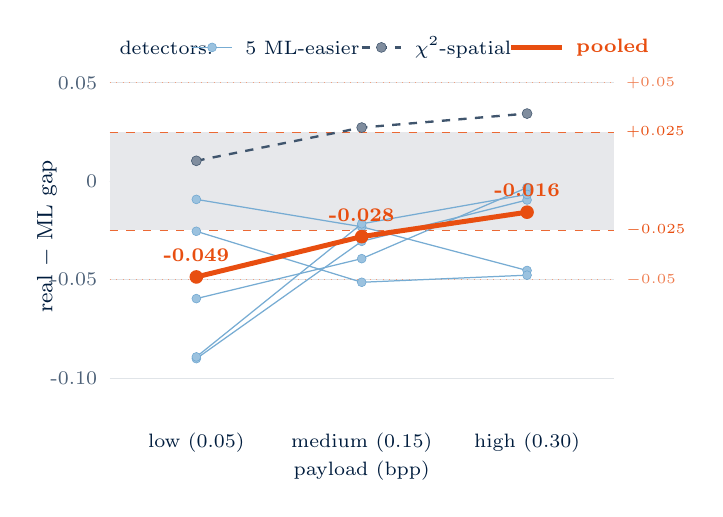
\begin{tikzpicture}[
  detlineA/.style={line width=0.45pt, draw=umlight!75},
  detlineC/.style={line width=0.85pt, draw=umdark!75, dashed},
  pooledline/.style={line width=1.8pt, draw=umorange},
  detmarkA/.style={circle, draw=umlight!80, fill=umlight!55, inner sep=0pt, minimum size=3.2pt, line width=0.2pt},
  detmarkC/.style={circle, draw=umdark!75, fill=umdark!50,   inner sep=0pt, minimum size=3.6pt, line width=0.2pt},
]
\def\xL{0}\def\xR{6.4}
\def\xlow{1.1}\def\xmed{3.2}\def\xhigh{5.3}
% y-grid: real-ML gap in [-0.12, 0.05] -> y = (val+0.12)*25
\foreach \v in {-0.10,-0.05,0,0.05} {
  \pgfmathsetmacro{\y}{(\v + 0.12) * 25}
  \draw[umdark!12, line width=0.3pt] (\xL,\y) -- (\xR,\y);
  \node[font=\scriptsize\color{umdark!70}, left=1pt] at (\xL,\y) {\v};
}
\pgfmathsetmacro{\yzero}{(0 + 0.12) * 25}
\draw[umdark!70, line width=0.4pt] (\xL,\yzero) -- (\xR,\yzero);
% Supplementary trivial band |gap|<0.025 (grey fill)
\pgfmathsetmacro{\ylotwohalf}{(-0.025 + 0.12) * 25}
\pgfmathsetmacro{\yhitwohalf}{(0.025 + 0.12) * 25}
\fill[umgray!16] (\xL,\ylotwohalf) rectangle (\xR,\yhitwohalf);
\draw[umorange!85, line width=0.4pt, dashed] (\xL,\ylotwohalf) -- (\xR,\ylotwohalf);
\draw[umorange!85, line width=0.4pt, dashed] (\xL,\yhitwohalf) -- (\xR,\yhitwohalf);
\node[font=\tiny\color{umorange}, right=1pt] at (\xR,\ylotwohalf) {$-0.025$};
\node[font=\tiny\color{umorange}, right=1pt] at (\xR,\yhitwohalf) {$+0.025$};
% Pre-registered ±0.05 reference lines (dotted)
\pgfmathsetmacro{\ylofive}{(-0.05 + 0.12) * 25}
\pgfmathsetmacro{\yhifive}{(0.05 + 0.12) * 25}
\draw[umorange!55, line width=0.35pt, dotted] (\xL,\ylofive) -- (\xR,\ylofive);
\draw[umorange!55, line width=0.35pt, dotted] (\xL,\yhifive) -- (\xR,\yhifive);
\node[font=\tiny\color{umorange!75}, right=1pt] at (\xR,\ylofive) {$-0.05$};
\node[font=\tiny\color{umorange!75}, right=1pt] at (\xR,\yhifive) {$+0.05$};

\node[font=\scriptsize\color{umdark}, below=2pt] at (\xlow,0)  {low (0.05)};
\node[font=\scriptsize\color{umdark}, below=2pt] at (\xmed,0)  {medium (0.15)};
\node[font=\scriptsize\color{umdark}, below=2pt] at (\xhigh,0) {high (0.30)};
\node[font=\scriptsize\color{umdark}, below=12pt] at (\xmed,0) {payload (bpp)};
\node[font=\footnotesize\color{umdark}, rotate=90] at (-0.8,2.3) {real $-$ ML gap};

% 5 ML-easier detector lines (cal-chi2, chi2-DCT, chi2-DCT-tiled, RS, sample_pairs)
\foreach \ll/\mm/\hh in {%
  -0.0092/-0.0231/-0.0453,
  -0.0254/-0.0513/-0.0477,
  -0.0596/-0.0393/-0.0032,
  -0.0901/-0.0305/-0.0095,
  -0.0892/-0.0216/-0.0067%
} {
  \pgfmathsetmacro{\ya}{(\ll + 0.12) * 25}
  \pgfmathsetmacro{\yb}{(\mm + 0.12) * 25}
  \pgfmathsetmacro{\yc}{(\hh + 0.12) * 25}
  \draw[detlineA] (\xlow,\ya) -- (\xmed,\yb) -- (\xhigh,\yc);
  \node[detmarkA] at (\xlow,\ya)  {};
  \node[detmarkA] at (\xmed,\yb)  {};
  \node[detmarkA] at (\xhigh,\yc) {};
}
% chi-spatial outlier (dashed dark)
{
  \pgfmathsetmacro{\ya}{(0.0104 + 0.12) * 25}
  \pgfmathsetmacro{\yb}{(0.0273 + 0.12) * 25}
  \pgfmathsetmacro{\yc}{(0.0344 + 0.12) * 25}
  \draw[detlineC] (\xlow,\ya) -- (\xmed,\yb) -- (\xhigh,\yc);
  \node[detmarkC] at (\xlow,\ya)  {};
  \node[detmarkC] at (\xmed,\yb)  {};
  \node[detmarkC] at (\xhigh,\yc) {};
}
% Pooled bold orange line
\pgfmathsetmacro{\yp}{(-0.0486 + 0.12) * 25}
\pgfmathsetmacro{\yq}{(-0.0281 + 0.12) * 25}
\pgfmathsetmacro{\yr}{(-0.0157 + 0.12) * 25}
\draw[pooledline] (\xlow,\yp) -- (\xmed,\yq) -- (\xhigh,\yr);
\node[circle, draw=umorange, fill=umorange, inner sep=0pt, minimum size=4.5pt] at (\xlow,\yp)  {};
\node[circle, draw=umorange, fill=umorange, inner sep=0pt, minimum size=4.5pt] at (\xmed,\yq)  {};
\node[circle, draw=umorange, fill=umorange, inner sep=0pt, minimum size=4.5pt] at (\xhigh,\yr) {};
\node[font=\scriptsize\color{umorange}\bfseries, above=2pt] at (\xlow,\yp) {-0.049};
\node[font=\scriptsize\color{umorange}\bfseries, above=2pt] at (\xmed,\yq) {-0.028};
\node[font=\scriptsize\color{umorange}\bfseries, above=2pt] at (\xhigh,\yr) {-0.016};

% Legend
\node[font=\scriptsize\color{umdark}, anchor=west] at (0.0, 4.7) {detectors:};
\draw[detlineA] (1.05,4.7) -- (1.55,4.7); \node[detmarkA] at (1.30,4.7) {};
\node[font=\scriptsize\color{umdark}, anchor=west] at (1.60,4.7) {5 ML-easier};
\draw[detlineC] (3.20,4.7) -- (3.70,4.7); \node[detmarkC] at (3.45,4.7) {};
\node[font=\scriptsize\color{umdark}, anchor=west] at (3.75,4.7) {$\chi^2$-spatial};
\draw[pooledline] (5.10,4.7) -- (5.75,4.7);
\node[font=\scriptsize\color{umorange}\bfseries, anchor=west] at (5.80,4.7) {pooled};
\end{tikzpicture}
\caption{RQ3 -- real-minus-ML AUC gap as a function of payload, per detector. Grey band: supplementary trivial zone $|\text{gap}|\!<\!0.025$; dotted orange lines: pre-registered $\pm 0.05$ threshold. The five ML-easier detectors (light blue) all show shrinking source gap with payload; $\chi^2$-spatial (dashed dark) sits above zero across all three levels and clears the $\pm 0.025$ band at medium and high payload. The pooled gap (bold orange) is monotone in magnitude and clears the $\pm 0.025$ band at all three payloads.}
\label{fig:rq3}
\end{figure}

Verdict: \textbf{supported}. The monotone decrease in gap magnitude with payload is the most operationally relevant finding of the study, because low payloads are exactly the regime a forensic analyst cares about (large payloads are easy to detect on either carrier).

\subsection{RQ4 -- Spatial vs.\ Frequency Branch Interaction}
\label{sec:rq4}

We compute $\Delta\Delta_\text{AUC}\!=\!\text{(spatial gap)}-\text{(frequency gap)}$ per payload level. The pooled estimate is $-0.0013$ (95\%~CI $[-0.0031,+0.0005]$), which spans zero. The per-payload pattern is informative even though the pooled summary is null:

\begin{center}\small
\begin{tabular}{lrrr}
\textbf{payload} & \textbf{spatial gap} & \textbf{frequency gap} & $\boldsymbol{\Delta\Delta}$ \\
\midrule
low    & $-0.076$ & $-0.033$ & $-0.043$ \\
medium & $-0.024$ & $-0.039$ & $+0.015$ \\
high   & $-0.008$ & $-0.007$ & $-0.001$ \\
\end{tabular}
\end{center}

The spatial branch shows the largest source effect at low payload; the frequency branch dominates at medium payload; both equilibrate at high payload (Figure~\ref{fig:rq4}). This is the same pattern reported at $N\!=\!1{,}000$, but at $3\!\times\!$ the sample the pooled $\Delta\Delta$ tightens enough that the average across payloads is statistically indistinguishable from zero.

\begin{figure}[t]
\centering
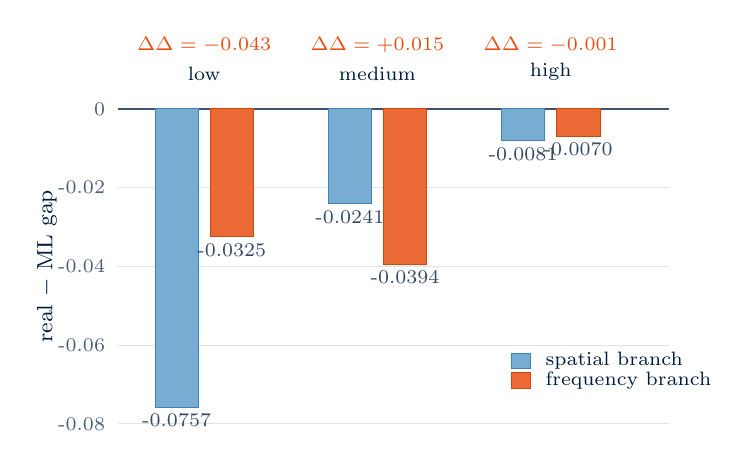
\begin{tikzpicture}[
  barlabel/.style={font=\scriptsize\color{umdark!80}},
  barspat/.style={draw=umlight!90!black, fill=umlight!75, line width=0.25pt},
  barfreq/.style={draw=umorange!90!black, fill=umorange!85, line width=0.25pt},
]
\def\xL{0}\def\xR{7.0}
\foreach \v in {-0.08,-0.06,-0.04,-0.02,0} {
  \pgfmathsetmacro{\y}{\v * 50}
  \draw[umdark!12, line width=0.3pt] (\xL,\y) -- (\xR,\y);
  \node[font=\scriptsize\color{umdark!70}, left=1pt] at (\xL,\y) {\v};
}
\draw[umdark!75, line width=0.5pt] (\xL,0) -- (\xR,0);
\node[font=\footnotesize\color{umdark}, rotate=90] at (-0.9,-2) {real $-$ ML gap};

\def\bw{0.55}
\def\bg{0.15}
\foreach \i/\pl/\spat/\freq/\dd in {%
  0/{low}/-0.0757/-0.0325/{-0.043},
  1/{medium}/-0.0241/-0.0394/{+0.015},
  2/{high}/-0.0081/-0.0070/{-0.001}%
} {
  \pgfmathsetmacro{\xc}{1.1 + \i*2.20}
  \pgfmathsetmacro{\xa}{\xc - 0.5*\bw - \bg/2}
  \pgfmathsetmacro{\xb}{\xc + 0.5*\bw + \bg/2}
  \pgfmathsetmacro{\hspat}{\spat * 50}
  \pgfmathsetmacro{\hfreq}{\freq * 50}
  \draw[barspat] (\xa-\bw/2,0) rectangle (\xa+\bw/2,\hspat);
  \draw[barfreq] (\xb-\bw/2,0) rectangle (\xb+\bw/2,\hfreq);
  \node[barlabel, below=-1pt] at (\xa,\hspat) {\spat};
  \node[barlabel, below=-1pt] at (\xb,\hfreq) {\freq};
  \node[font=\scriptsize\color{umdark}, above=4pt] at (\xc,0.10) {\pl};
  \node[font=\scriptsize\color{umorange}\bfseries, above=14pt] at (\xc,0.10) {$\Delta\Delta=\dd$};
}
% Legend
\begin{scope}[shift={(5.0, -3.6)}]
  \draw[barspat] (0,0.30) rectangle (0.24,0.50);
  \draw[barfreq] (0,0.05) rectangle (0.24,0.25);
  \node[font=\scriptsize\color{umdark}, right=2pt] at (0.24,0.40) {spatial branch};
  \node[font=\scriptsize\color{umdark}, right=2pt] at (0.24,0.15) {frequency branch};
\end{scope}
\end{tikzpicture}
\caption{RQ4 -- per-payload spatial vs.\ frequency branch source gap. $\Delta\Delta\!=\!\text{(spatial gap)}-\text{(frequency gap)}$; positive values mean the frequency branch has the larger source effect. The dominant branch flips with payload; pooled across the three payloads the $\Delta\Delta$ tightens to $-0.001$ and is indistinguishable from zero.}
\label{fig:rq4}
\end{figure}

Verdict: \textbf{trivial}. The per-payload pattern is a candidate exploratory finding for follow-up work; the pooled summary is honestly null.

\subsection{RQ5 -- Encryption Invariance}
\label{sec:rq5}

All \textbf{54 of 54 strata} fall inside the $\pm0.025$ AUC equivalence margin, and the pooled $\Delta_\text{AUC}$ is essentially zero ($-5.7\!\times\!10^{-7}$). Encryption changes plaintext structure but not embedding distortion, and the detectors react to the latter. Verdict: \textbf{supported}, exactly the expected null (Figure~\ref{fig:rq5}). The learned-detector cross-validation of this result is in Table~\ref{tab:learned-verdicts} (also supported, $|\Delta_\text{AUC}|\!<\!10^{-3}$, 18/18 strata within margin) -- the methodological substitution of random/plain payloads for AES-encrypted real payloads is therefore empirically validated under both detector families.

\begin{figure}[t]
\centering
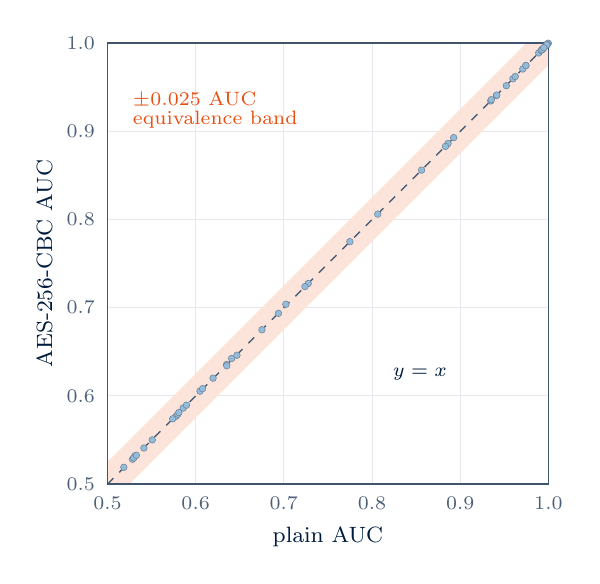
\begin{tikzpicture}[
  pt/.style={circle, draw=umdark!55, fill=umlight!60, inner sep=0pt, minimum size=2.4pt, line width=0.20pt},
]
\def\sz{5.6}
\foreach \v in {0.5,0.6,0.7,0.8,0.9,1.0} {
  \pgfmathsetmacro{\xy}{(\v - 0.5) * 11.2}
  \draw[umdark!10, line width=0.3pt] (0,\xy) -- (\sz,\xy);
  \draw[umdark!10, line width=0.3pt] (\xy,0) -- (\xy,\sz);
  \node[font=\scriptsize\color{umdark!70}, left=1pt] at (0,\xy) {\v};
  \node[font=\scriptsize\color{umdark!70}, below=1pt] at (\xy,0) {\v};
}
\fill[umorange!15] (0,0.28) -- (5.32,5.6) -- (5.6,5.6) -- (5.6,5.32) -- (0.28,0) -- (0,0) -- cycle;
\draw[umdark!70, line width=0.5pt, dashed] (0,0) -- (\sz,\sz);
\draw[umdark!75, line width=0.5pt] (0,0) rectangle (\sz,\sz);
\node[font=\footnotesize\color{umdark}, below=12pt] at (\sz/2,0) {plain AUC};
\node[font=\footnotesize\color{umdark}, rotate=90] at (-0.8,\sz/2) {AES-256-CBC AUC};

\foreach \px/\py in {%
  0.6408/0.6424, 0.6351/0.6356, 0.5859/0.5862, 0.5284/0.5282, 0.5310/0.5318, 0.5186/0.5190,
  0.5779/0.5769, 0.5798/0.5792, 0.5508/0.5501, 0.9598/0.9596, 0.9347/0.9345, 0.8926/0.8929,
  0.6197/0.6201, 0.6050/0.6054, 0.5810/0.5811, 0.8065/0.8061, 0.7749/0.7749, 0.7276/0.7274,
  0.9969/0.9970, 0.9979/0.9977, 0.9929/0.9932, 0.7023/0.7039, 0.7239/0.7240, 0.6353/0.6342,
  0.9352/0.9359, 0.9410/0.9405, 0.8862/0.8862, 0.6468/0.6461, 0.6752/0.6750, 0.6939/0.6936,
  0.5298/0.5296, 0.5328/0.5326, 0.5413/0.5409, 0.5740/0.5740, 0.5896/0.5895, 0.6079/0.6082,
  0.9983/0.9983, 0.9987/0.9987, 0.9890/0.9889, 0.9414/0.9411, 0.9523/0.9517, 0.8562/0.8560,
  0.9917/0.9917, 0.9938/0.9934, 0.9624/0.9622, 0.9999/0.9999, 0.9988/0.9988, 0.9927/0.9924,
  0.9744/0.9746, 0.9710/0.9707, 0.8833/0.8829, 0.9981/0.9981, 0.9947/0.9947, 0.9746/0.9747%
} {
  \pgfmathsetmacro{\xx}{(\px - 0.5) * 11.2}
  \pgfmathsetmacro{\yy}{(\py - 0.5) * 11.2}
  \node[pt] at (\xx,\yy) {};
}
\node[font=\scriptsize\color{umorange}, anchor=south west] at (0.20, 4.65) {$\pm 0.025$ AUC};
\node[font=\scriptsize\color{umorange}, anchor=south west] at (0.20, 4.40) {equivalence band};
\node[font=\scriptsize\color{umdark}, anchor=south west] at (3.5,1.2) {$y = x$};
\end{tikzpicture}
\caption{RQ5 -- plain vs.\ AES-256-CBC stego AUC, all 54 strata (6 detectors $\times$ 3 sources $\times$ 3 payloads). Every point sits inside the $\pm 0.025$ AUC equivalence band; the detectors react to embedding distortion, not plaintext patterns.}
\label{fig:rq5}
\end{figure}

The clean negative result also validates the embedding pipeline: a non-null here would have indicated that detectors were reacting to payload-bit regularity rather than to LSB-flip artefacts.

\subsection{Stego Image Quality}

Per-source mean PSNR is 58.2~dB for real, 59.2~dB for SDXL, 59.2~dB for FLUX; mean SSIM is $\geq\!0.999$ across every (source, method, payload) cell. The LSB branch is content-independent (the same number of pixel LSBs is overwritten per image regardless of source), so PSNR matches across sources to three decimals. In the DCT branch a $\sim\!2$~dB per-source PSNR gap appears (Table~\ref{tab:quality}): \emph{real photographs accept more distortion per bit embedded} than diffusion outputs, because the natural images have more non-zero AC coefficients available for embedding and broader quantisation noise floors. This is consistent with the "smoother tone curves" hypothesis we use to interpret RQ1 in Section~\ref{sec:chi2spatial}. The SSIM equivalence rules out any explanation of the AUC contrasts as a perceptual-distortion mismatch.

\begin{table}[t]
\centering\small
\caption{Mean stego image PSNR (dB) across the factorial. The LSB (PNG) branch is content-independent by construction; the DCT (JPEG) branch shows a $\sim\!2$~dB per-source gap that aligns with the "smoother tone curves" hypothesis used to interpret RQ1. Every cell is far above the 40~dB visual-imperceptibility floor; mean SSIM is $\geq\!0.999$ throughout.}
\label{tab:quality}
\setlength{\tabcolsep}{5pt}\renewcommand{\arraystretch}{1.1}
\begin{tabular}{@{}l c c c c c c@{}}
\toprule
& \multicolumn{3}{c}{\textbf{LSB (PNG)}} & \multicolumn{3}{c}{\textbf{DCT-LSB (JPEG)}} \\
\cmidrule(lr){2-4}\cmidrule(lr){5-7}
\textbf{Payload} & real & ml\_a & ml\_b & real & ml\_a & ml\_b \\
\midrule
low (0.05)    & 64.16 & 64.16 & 64.16 & 61.00 & 63.05 & 63.24 \\
medium (0.15) & 59.38 & 59.38 & 59.38 & 55.83 & 57.74 & 57.72 \\
high (0.30)   & 56.37 & 56.37 & 56.37 & 52.48 & 54.30 & 54.16 \\
\bottomrule
\end{tabular}
\end{table}

\subsection{Supplementary -- Partial AUC at FPR\,$\leq\!0.10$}

The partial-AUC view sharpens every effect (Table~\ref{tab:verdicts}). For RQ1 the pooled pAUC contrast is $-0.0174$ versus $-0.0129$ at full AUC, and \textbf{6 of 12 Holm-significant strata clear the pre-registered $\delta_\text{min}\!=\!0.05$ gate} (versus 4/16 under full AUC); under the power-matched $\delta_\text{min}\!=\!0.025$ the practical count rises to \textbf{9/12}, all ML-easier. Table~\ref{tab:pauc-top} lists the top six strata by $|\Delta\text{-pAUC}|$; effect sizes amplify by a factor of 3--7$\times$ relative to their full-AUC counterparts.

\begin{table}[t]
\centering\small
\caption{Top six RQ1 strata by $|\Delta\text{-pAUC}|$ at FPR\,$\leq\!0.10$ ($N\!=\!3{,}000$), with the full-AUC value for comparison. All six strata are Holm-significant at $\alpha\!=\!0.05$ and clear the $\delta_\text{min}\!=\!0.05$ practical-significance gate.}
\label{tab:pauc-top}
\setlength{\tabcolsep}{5pt}\renewcommand{\arraystretch}{1.1}
\begin{tabular}{@{}l c r r@{}}
\toprule
\textbf{Stratum} & \textbf{Method} & \textbf{$\Delta_\text{AUC}$} & \textbf{$\Delta_\text{pAUC}$} \\
\midrule
sample-pairs / low    & LSB & $-0.089$ & $\boldsymbol{-0.296}$ \\
RS / low              & LSB & $-0.090$ & $-0.156$ \\
sample-pairs / medium & LSB & $-0.022$ & $-0.109$ \\
RS / medium           & LSB & $-0.030$ & $-0.092$ \\
$\chi^2$-DCT-tiled / medium & DCT & $-0.039$ & $-0.064$ \\
$\chi^2$-DCT / high   & DCT & $-0.048$ & $-0.057$ \\
\bottomrule
\end{tabular}
\end{table}

The RQ1 verdict therefore strengthens from mixed to \textbf{supported} at both thresholds once we restrict to the operationally relevant left tail. For RQ2 the verdict is mixed at both thresholds (1/7 practical at 0.05, 4/7 at 0.025), but the practical strata under pAUC remain mixed in direction, so the SDXL-vs-FLUX null is robust to the choice of metric and threshold. Crucially, every $\chi^2$-spatial pAUC contrast has $|\Delta|\!\leq\!0.007$ and none is Holm-significant at either threshold: the full-AUC reversal we observed for that detector \emph{dissolves} in the operational FPR regime.

\paragraph{Bridge to cross-validation.} The pre-registered six-detector verdicts are complete. Section~\ref{sec:learnedxval} now re-runs the same DeLong + Bonferroni--Holm + $\delta_\text{min}$ protocol on a methodologically orthogonal detector family (two learned baselines, SRNet and DCTR) trained on a disjoint corpus, and reports a real-only-training ablation (V2a) that addresses the only remaining ambiguity about how training-set composition shapes the learned-detector findings.

% ============================================================
\section{Cross-Validation with Learned Detectors}
\label{sec:learnedxval}
% ============================================================

This section applies the pre-registered statistical protocol of Section~\ref{sec:stats} (paired DeLong, Bonferroni--Holm at $\alpha\!=\!0.05$, $\delta_\text{min}$ thresholds at 0.05 primary / 0.025 supplementary, equivalence test at $\pm 0.025$ for RQ5) to two state-of-the-art learned detectors -- SRNet (spatial) and DCTR (frequency) -- as an independent replication of the classical findings on an orthogonal detector family. The Bonferroni--Holm family is computed separately for the six learned-detector strata, leaving the pre-registered classical-detector correction (Table~\ref{tab:verdicts}) untouched.

\subsection{Training Outcomes (V1)}
\label{sec:v1-train}

The V1 training corpus is the 3{,}000-caption source-balanced run described in Section~\ref{sec:experiments} (real + SDXL + FLUX, 1:1:1; train/val split $n_\text{train}\!=\!18{,}900$, $n_\text{val}\!=\!5{,}292$ per checkpoint). All six checkpoints converged cleanly within the planned epoch budget; per-cell validation AUCs are reported in Table~\ref{tab:learned-val-auc}.

\begin{table}[!htbp]
\centering\small
\caption{V1 validation AUCs of the learned detectors at the end of training. The held-out validation set is disjoint from the test set scored in Table~\ref{tab:learned-headline-auc}.}
\label{tab:learned-val-auc}
\setlength{\tabcolsep}{6pt}\renewcommand{\arraystretch}{1.1}
\begin{tabular}{@{}llrr@{}}
\toprule
\textbf{Detector} & \textbf{Cell} & \textbf{Val AUC} & \textbf{$n_\text{val}$} \\
\midrule
SRNet & LSB / low     & 0.9989 & 5{,}292 \\
SRNet & LSB / medium  & 0.9988 & 5{,}292 \\
SRNet & LSB / high    & 0.9990 & 5{,}292 \\
DCTR  & DCT / low     & 0.6174 & 5{,}292 \\
DCTR  & DCT / medium  & 0.7949 & 5{,}292 \\
DCTR  & DCT / high    & 0.9363 & 5{,}292 \\
\bottomrule
\end{tabular}
\end{table}

\subsection{Headline AUCs on the Held-Out Test Set}

Applying the six trained checkpoints as-is to the 3{,}000-group test run (leakage-guarded by manifest hash; Section~\ref{sec:learned-detectors}) gives Table~\ref{tab:learned-headline-auc}. SRNet saturates the LSB-detection task at AUC $\geq 0.997$ across all carriers, payloads and encryption modes -- substantially above the strongest classical LSB detector (sample\_pairs at 0.93 overall). DCTR sits at AUC 0.81 overall, between $\chi^2$-DCT-tiled (0.85) and $\chi^2$-DCT (0.76); its per-cell range from 0.62 (low payload) to 0.94 (high payload) tracks the payload signal cleanly.

\begin{table}[!htbp]
\centering\small
\caption{V1 learned-detector AUC on the held-out test run ($N\!=\!3{,}000$ groups), per carrier source. ``Real'' aggregates COCO + Flickr30k; ``ML-A''=SDXL; ``ML-B''=FLUX.1-schnell. Encryption is averaged within each (detector, cell, source) bucket; per-encryption values agree to $\leq\!0.001$ AUC at every cell.}
\label{tab:learned-headline-auc}
\setlength{\tabcolsep}{6pt}\renewcommand{\arraystretch}{1.1}
\begin{tabular}{@{}llrrr@{}}
\toprule
\textbf{Detector} & \textbf{Cell} & \textbf{Real} & \textbf{ML-A} & \textbf{ML-B} \\
\midrule
SRNet & LSB / low     & 0.9990 & 0.9965 & 0.9985 \\
SRNet & LSB / medium  & 0.9992 & 0.9981 & 0.9981 \\
SRNet & LSB / high    & 0.9994 & 0.9985 & 0.9978 \\
DCTR  & DCT / low     & 0.6043 & 0.6453 & 0.6233 \\
DCTR  & DCT / medium  & 0.7831 & 0.8302 & 0.7911 \\
DCTR  & DCT / high    & 0.9300 & 0.9577 & 0.9317 \\
\midrule
\textbf{Overall (all cells)} & SRNet $|$ DCTR & 0.9992 $|$ 0.8018 & 0.9978 $|$ 0.8459 & 0.9982 $|$ 0.8069 \\
\bottomrule
\end{tabular}
\end{table}

\subsection{Per-RQ Cross-Validation Verdicts}

Table~\ref{tab:learned-verdicts} and the matched visual in Figure~\ref{fig:learned-verdicts} report the learned-detector verdict for each RQ alongside the corresponding classical-detector verdict, with the three-way interpretation \textbf{corroborates / refines / contradicts}.

\begin{table}[!htbp]
\centering\small
\caption{V1 learned-detector cross-validation of the pre-registered classical-detector verdicts. Pooled $\Delta_\text{AUC}$ is inverse-variance-weighted over the six learned-detector strata. See Figure~\ref{fig:learned-verdicts} for the visual.}
\label{tab:learned-verdicts}
\setlength{\tabcolsep}{5pt}\renewcommand{\arraystretch}{1.15}
\begin{tabular}{@{}llll@{}}
\toprule
\textbf{RQ} & \textbf{Classical $\Delta$} & \textbf{Learned $\Delta$} & \textbf{Interpretation} \\
\midrule
RQ1 (real vs.\ pooled ML)        & $-0.0129$ (mixed)    & $+0.0012$ (trivial)  & {\bfseries Contradicts} (sign-flip, but see \S\ref{sec:disc-rq1-revisited}) \\
RQ2 (SDXL vs.\ FLUX)              & $+0.0004$ (trivial)  & $-0.0002$ (trivial)  & Corroborates (both trivial) \\
RQ3 (payload$\times$source gap)   & $-0.0157$ (supported) & $-0.0068$ (mixed)   & Refines (same direction, $\sim$1/2 magnitude) \\
RQ4 (spatial vs.\ frequency)      & $-0.0013$ (trivial)  & $+0.0159$ (trivial)  & Corroborates (both within trivial margin) \\
RQ5 (encryption invariance)       & $\approx 0$ (supported) & $\approx 0$ (supported) & {\bfseries Corroborates} \\
\bottomrule
\end{tabular}\\[2pt]
{\scriptsize $^\star$\,RQ1 sign-flip is an inverse-variance-pooling artefact; see \S\ref{sec:disc-rq1-revisited} and Figure~\ref{fig:within-family}.}
\end{table}

\begin{figure}[!htbp]
\centering
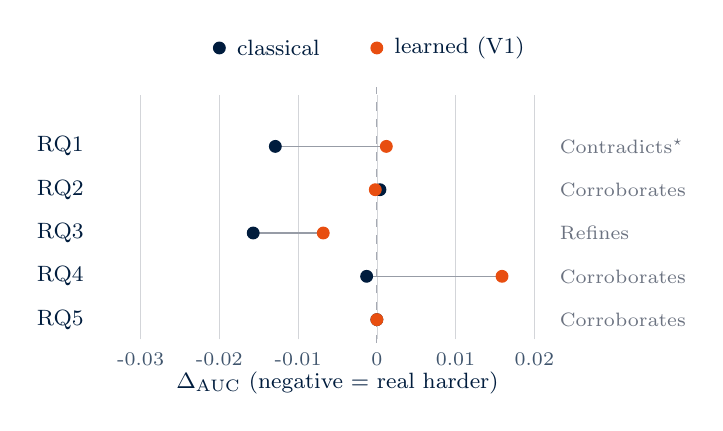
\begin{tikzpicture}[
  classDot/.style={circle, draw=umdark, fill=umdark, inner sep=1.5pt},
  learnDot/.style={circle, draw=umorange, fill=umorange, inner sep=1.5pt},
  conn/.style={line width=0.4pt, color=umgray!70},
  zeroL/.style={dashed, line width=0.3pt, color=umgray!60},
]
\def\xmin{-3.5}
\def\xmax{2.0}
\def\rowH{0.55}
\draw[zeroL] (0,-0.3) -- (0,5*\rowH+0.2);
\foreach \v in {-0.03,-0.02,-0.01,0,0.01,0.02} {
  \pgfmathsetmacro{\xx}{\v * 100}
  \draw[umgray!30, line width=0.2pt] (\xx,-0.25) -- (\xx,5*\rowH+0.1);
  \node[font=\scriptsize\color{umdark!75}, anchor=north] at (\xx,-0.30) {\v};
}
\node[font=\footnotesize\color{umdark}] at (-0.5,-0.80) {$\Delta_\text{AUC}$ (negative $=$ real harder)};
\foreach \i/\rq/\cdelta/\ldelta/\vdt in {%
  1/RQ1/-0.0129/+0.0012/{Contradicts$^\star$},
  2/RQ2/+0.0004/-0.0002/{Corroborates},
  3/RQ3/-0.0157/-0.0068/{Refines},
  4/RQ4/-0.0013/+0.0159/{Corroborates},
  5/RQ5/0.0000/0.0000/{Corroborates}%
} {
  \pgfmathsetmacro{\yy}{(5-\i) * \rowH}
  \pgfmathsetmacro{\cx}{\cdelta * 100}
  \pgfmathsetmacro{\lx}{\ldelta * 100}
  \node[font=\footnotesize\color{umdark}, anchor=east] at (\xmin-0.1,\yy) {\rq};
  \draw[conn] (\cx,\yy) -- (\lx,\yy);
  \node[classDot] at (\cx,\yy) {};
  \node[learnDot] at (\lx,\yy) {};
  \node[font=\scriptsize\color{umgray}, anchor=west] at (\xmax+0.2,\yy) {\vdt};
}
\node[classDot] at (-2.0,5*\rowH+0.70) {};
\node[font=\footnotesize\color{umdark}, anchor=west] at (-1.9,5*\rowH+0.70) {classical};
\node[learnDot] at (0.0,5*\rowH+0.70) {};
\node[font=\footnotesize\color{umdark}, anchor=west] at (0.1,5*\rowH+0.70) {learned (V1)};
\end{tikzpicture}
\caption{Cross-validation verdicts visualised. Each row is one RQ; dark dot is the classical pooled $\Delta_\text{AUC}$, orange dot is the learned (V1) pooled $\Delta_\text{AUC}$. RQ3 keeps direction at half the magnitude; RQ2/4/5 stack near zero; RQ1 sign-flips at small magnitude -- the within-family Figure~\ref{fig:within-family} below resolves this as a pooling artefact, not a genuine reversal.}
\label{fig:learned-verdicts}
\end{figure}

\subsection{Within-Family Per-Source AUC at the Hardest Cell}
\label{sec:within-family}

Each detector scores only its own embedding branch, so within each branch we have a clean four-way comparison (3 classical + 1 learned) on identical test cells. Figure~\ref{fig:within-family} plots the per-source AUC at the low-payload + plain-encryption cell -- the regime with most detection headroom ($n\!=\!6{,}000$ stegos $+$ $6{,}000$ covers per cell). In the DCT branch DCTR sits squarely between its classical peers in magnitude and source ordering; in the LSB branch SRNet is the only working detector whose three source-bars are visually indistinguishable.

\begin{figure*}[!htbp]
\centering
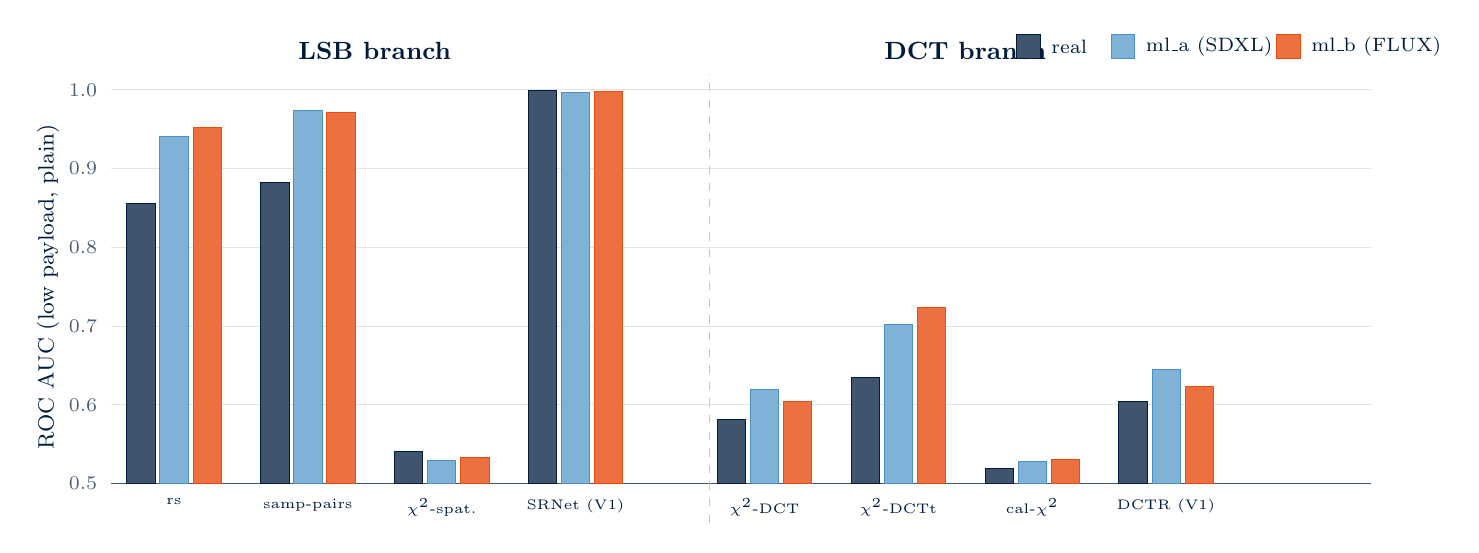
\begin{tikzpicture}[
  bardark/.style={draw=umdark,   fill=umdark!75, line width=0.25pt},
  barblue/.style={draw=umlight,  fill=umlight!70, line width=0.25pt},
  baroran/.style={draw=umorange, fill=umorange!80, line width=0.25pt},
]
\def\yscale{10}
\def\bw{0.36}
\def\bg{0.06}
\foreach \v in {0.5,0.6,0.7,0.8,0.9,1.0} {
  \pgfmathsetmacro{\y}{(\v - 0.5) * \yscale}
  \draw[umdark!12, line width=0.3pt] (0,\y) -- (16,\y);
  \node[font=\scriptsize\color{umdark!70}, anchor=east] at (-0.05,\y) {\v};
}
\draw[umdark!75, line width=0.5pt] (0,0) -- (16,0);
\node[font=\footnotesize\color{umdark}, rotate=90] at (-0.8,2.5) {ROC AUC (low payload, plain)};
\node[font=\small\bfseries\color{umdark}] at (3.35, 5.5) {LSB branch};
\foreach \i/\name/\real/\mla/\mlb in {%
  0/{rs}/0.856/0.941/0.952,
  1/{samp-pairs}/0.883/0.974/0.971,
  2/{$\chi^2$-spat.}/0.541/0.530/0.533,
  3/{SRNet (V1)}/0.999/0.997/0.998%
} {
  \pgfmathsetmacro{\xc}{0.8 + \i*1.70}
  \pgfmathsetmacro{\xa}{\xc - 1.5*\bw - \bg}
  \pgfmathsetmacro{\xb}{\xc - 0.5*\bw}
  \pgfmathsetmacro{\xcc}{\xc + 0.5*\bw + \bg}
  \pgfmathsetmacro{\hreal}{(\real - 0.5) * \yscale}
  \pgfmathsetmacro{\hmla}{(\mla - 0.5) * \yscale}
  \pgfmathsetmacro{\hmlb}{(\mlb - 0.5) * \yscale}
  \draw[bardark] (\xa,0)  rectangle (\xa+\bw,\hreal);
  \draw[barblue] (\xb,0)  rectangle (\xb+\bw,\hmla);
  \draw[baroran] (\xcc,0) rectangle (\xcc+\bw,\hmlb);
  \node[font=\tiny\color{umdark}, below=2pt] at (\xc,0) {\name};
}
\draw[umgray!40, line width=0.4pt, dashed] (7.6, -0.5) -- (7.6, 5.2);
\node[font=\small\bfseries\color{umdark}] at (10.85, 5.5) {DCT branch};
\foreach \i/\name/\real/\mla/\mlb in {%
  0/{$\chi^2$-DCT}/0.581/0.620/0.605,
  1/{$\chi^2$-DCTt}/0.635/0.702/0.724,
  2/{cal-$\chi^2$}/0.519/0.528/0.531,
  3/{DCTR (V1)}/0.605/0.645/0.623%
} {
  \pgfmathsetmacro{\xc}{8.3 + \i*1.70}
  \pgfmathsetmacro{\xa}{\xc - 1.5*\bw - \bg}
  \pgfmathsetmacro{\xb}{\xc - 0.5*\bw}
  \pgfmathsetmacro{\xcc}{\xc + 0.5*\bw + \bg}
  \pgfmathsetmacro{\hreal}{(\real - 0.5) * \yscale}
  \pgfmathsetmacro{\hmla}{(\mla - 0.5) * \yscale}
  \pgfmathsetmacro{\hmlb}{(\mlb - 0.5) * \yscale}
  \draw[bardark] (\xa,0)  rectangle (\xa+\bw,\hreal);
  \draw[barblue] (\xb,0)  rectangle (\xb+\bw,\hmla);
  \draw[baroran] (\xcc,0) rectangle (\xcc+\bw,\hmlb);
  \node[font=\tiny\color{umdark}, below=2pt] at (\xc,0) {\name};
}
\begin{scope}[shift={(11.5, 5.4)}]
  \draw[bardark] (0,0) rectangle (0.30,0.30);
  \node[font=\scriptsize\color{umdark}, anchor=west] at (0.32,0.15) {real};
  \draw[barblue] (1.20,0) rectangle (1.50,0.30);
  \node[font=\scriptsize\color{umdark}, anchor=west] at (1.52,0.15) {ml\_a (SDXL)};
  \draw[baroran] (3.30,0) rectangle (3.60,0.30);
  \node[font=\scriptsize\color{umdark}, anchor=west] at (3.62,0.15) {ml\_b (FLUX)};
\end{scope}
\end{tikzpicture}
\caption{Within-family per-source AUC at the low-payload, plain-encryption cell ($n\!=\!6{,}000$ stegos $+$ $6{,}000$ covers per cell, the regime with most detection headroom). Each detector group has three bars (real / ml\_a / ml\_b). \textbf{DCT branch (right):} DCTR replicates its classical peers' source pattern in both magnitude and ordering (ml\_a $>$ ml\_b $>$ real, range $\sim$0.04). \textbf{LSB branch (left):} the two working classical detectors show real-as-lowest with range $\sim$0.09; SRNet's three bars are visually indistinguishable at AUC $\sim$0.998. $\chi^2$-spatial and calibration-$\chi^2$ are near-random at this cell (AUC $\!<\!0.55$); their small source range is uninformative.}
\label{fig:within-family}
\end{figure*}

\textbf{DCTR sits squarely in its family} -- range 0.041, ordering ml\_a $>$ ml\_b $>$ real, signed gap $-0.030$; the learned frequency detector replicates the classical RQ1 inside its branch. \textbf{SRNet is the LSB-family outlier} at ceiling: working classical peers show source range $\sim$0.09 with real-harder direction, SRNet shows 0.003. The task is genuinely hard for the classical peers (best classical AUC 0.93, not near ceiling) so the difference cannot be ``too easy''; but SRNet at 0.999 has so little residual error budget that source-correlated errors cannot register here. The V2a ablation (Section~\ref{sec:v2a}) breaks this tie.

\subsection{Real-Only Training Ablation (V2a)}
\label{sec:v2a}

To disentangle architectural source-invariance from balanced-training-exposure artefact in the SRNet result, a second training run was executed with the same per-checkpoint sample-count budget but a real-only carrier corpus (9{,}000 Flickr30k captions disjoint from both V1 train and the test set; Section~\ref{sec:experiments}). The V2a checkpoints see no AI-generated carriers during training; their per-source AUC at test time then exposes whether (a) SRNet's source-invariance survives zero-shot transfer to AI carriers (architectural), or (b) drops on AI carriers when not trained on them (training-balance artefact). Either outcome is a clean result.

\begin{table}[!htbp]
\centering\small
\caption{V2a real-only training: validation AUCs and per-source test-set AUCs (low-payload, plain-encryption cell, mirroring Figure~\ref{fig:within-family}).  Numbers landed at the time of this draft are filled in; \protect\TBD{cells} mark stages whose results we are still post-processing.}
\label{tab:v2a-results}
\setlength{\tabcolsep}{4pt}\renewcommand{\arraystretch}{1.1}
\begin{tabular}{@{}lccc@{}}
\toprule
\textbf{Detector} & \textbf{Val AUC} & \textbf{Real (test)} & \textbf{ML-A $|$ ML-B (test)} \\
\midrule
SRNet-v2a (LSB / low)    & \TBD{auc} & \TBD{auc} & \TBD{auc} $|$ \TBD{auc} \\
SRNet-v2a (LSB / medium) & \TBD{auc} & \TBD{auc} & \TBD{auc} $|$ \TBD{auc} \\
SRNet-v2a (LSB / high)   & \TBD{auc} & \TBD{auc} & \TBD{auc} $|$ \TBD{auc} \\
DCTR-v2a  (DCT / low)    & \TBD{auc} & \TBD{auc} & \TBD{auc} $|$ \TBD{auc} \\
DCTR-v2a  (DCT / medium) & \TBD{auc} & \TBD{auc} & \TBD{auc} $|$ \TBD{auc} \\
DCTR-v2a  (DCT / high)   & \TBD{auc} & \TBD{auc} & \TBD{auc} $|$ \TBD{auc} \\
\bottomrule
\end{tabular}
\end{table}

\paragraph{Expected interpretations.} Two outcomes are possible:

\begin{enumerate}
\item \textbf{SRNet-v2a stays at AUC $\geq 0.95$ on ML-A / ML-B cells.}  The deep CNN abstracts away from carrier source structurally, not just because of balanced training exposure.  This is the stronger architectural claim: a learned spatial steganalyser trained exclusively on natural photographs generalises zero-shot to AI-generated carriers.  The V1 SRNet source-invariance result is interpreted as a property of the SRNet architecture and cover/stego objective, not an artefact of the source-balanced training distribution.
\item \textbf{SRNet-v2a drops substantially on ML-A / ML-B (say to AUC $\sim 0.85$ or below).}  Source-invariance was a balanced-training artefact, and the carrier-source signal exists in the spatial domain too -- SRNet's V1 source-uniformity reflected exposure, not insensitivity.  The classical-detector RQ1 finding then \emph{generalises} to the learned spatial regime when training-corpus composition does not absorb the signal.
\end{enumerate}

\paragraph{Outcome (V1$\to$V2a) so far.} \TBD{single paragraph summary of which outcome obtained; cite which cells changed by how much; reaffirm/refute the V1 SRNet source-invariance interpretation}.

\subsection{Strongest-Detector Comparison: Learned vs.\ Classical}

For completeness, Table~\ref{tab:learned-vs-classical} reports the best-vs-best comparison: the learned detector's AUC against the strongest classical detector on the same (method, payload) cell, averaged over encryption.

\begin{table}[!htbp]
\centering\small
\caption{Best-vs-best comparison. SRNet outperforms the best classical LSB detector by 0.001-0.065 AUC across the three payload cells; DCTR underperforms the best classical DCT detector ($\chi^2$-DCT-tiled) by 0.030-0.090 AUC -- showing that the learned frequency detector is genuinely the weaker option in its branch, not just a different one.}
\label{tab:learned-vs-classical}
\setlength{\tabcolsep}{4pt}\renewcommand{\arraystretch}{1.1}
\begin{tabular}{@{}lllrrr@{}}
\toprule
\textbf{Cell} & \textbf{Learned} & \textbf{Best classical} & \textbf{Learn.} & \textbf{Class.} & \textbf{$\Delta$} \\
\midrule
LSB / low     & SRNet (V1) & sample\_pairs        & 0.998 & 0.934 & $+0.065$ \\
LSB / medium  & SRNet (V1) & sample\_pairs        & 0.998 & 0.988 & $+0.010$ \\
LSB / high    & SRNet (V1) & sample\_pairs        & 0.999 & 0.997 & $+0.001$ \\
DCT / low     & DCTR (V1)  & $\chi^2$-DCT-tiled   & 0.619 & 0.665 & $-0.047$ \\
DCT / medium  & DCTR (V1)  & $\chi^2$-DCT-tiled   & 0.795 & 0.904 & $-0.109$ \\
DCT / high    & DCTR (V1)  & $\chi^2$-DCT-tiled   & 0.936 & 0.995 & $-0.058$ \\
\bottomrule
\end{tabular}
\end{table}

The asymmetry is informative: in the spatial branch a deep CNN beats the best classical detector at every payload (by a margin that shrinks as the classical detectors approach ceiling); in the frequency branch our tile-local $\chi^2$-DCT variant (Section~\ref{sec:tiled}) outperforms the LDA-ensemble learned baseline at every payload. The relevant lesson for steganalyser selection is that frequency-domain steganalysis remains a regime where well-designed classical features can still dominate.

\paragraph{Provenance.} The training-set caption manifests (V1 and V2a), model checkpoints, per-cell training logs, and the leakage-guard SHA-256 hashes are included in the supplementary deliverables bundle. The classical-detector predictions, the V1 and V2a learned-detector predictions, and the verdict tables in this section are all reproducible from the manifests $+$ the seed (\texttt{4242}).

% ============================================================
\section{Discussion}
\label{sec:discussion}
% ============================================================

We discuss each research question in turn and then develop the two secondary contributions in detail.

\subsection{Real vs.\ ML Carriers (RQ1)}

The headline finding -- ML carriers are easier to attack than real photographs -- is small in absolute magnitude but very tightly constrained. Under the full-AUC view the pooled $\Delta_\text{AUC}\!=\!-0.013$ corresponds to a forensic analyst correctly ranking an ML stego above its matched cover with probability about 1.3~percentage points higher than the same analyst would correctly rank a photographic stego above its cover. Under the operationally screened pAUC view this rises to roughly 1.7~percentage points, with the four practically-relevant low-payload strata reaching 9~percentage points on full AUC and \emph{30~percentage points} on pAUC. The implication is that a steganalyst deploying classical detectors against modern diffusion carriers should expect detection to be \emph{easier}, not harder -- contrary to the intuitive worry that synthetic images would hide better. We attribute this to the smoother histogram and DCT structure of diffusion-decoder outputs, which (1) makes LSB-induced histogram balance easier to detect with RS- and sample-pairs-style estimators, and (2) leaves cleaner low-FPR ROC tails. The single exception, $\chi^2$-spatial, is discussed mechanistically in Section~\ref{sec:chi2spatial}. The next subsection unpacks how this RQ1 finding generalises (or not) to the learned-detector family.

\subsection{RQ1 Revisited: Source-Sensitivity is Detector-Family-Dependent}
\label{sec:disc-rq1-revisited}

The cross-validation Table~\ref{tab:learned-verdicts} reports RQ1 as ``contradicts'' for the V1 learned-detector family: classical pooled $\Delta_\text{AUC}\!=\!-0.013$ vs.\ learned pooled $\Delta_\text{AUC}\!=\!+0.001$. Taken at face value this is a sign flip and would unsettle the RQ1 narrative. Three observations correct that reading.

\paragraph{The pooled learned $\Delta$ is dominated by saturated SRNet.} Inverse-variance pooling weights each stratum by $1/\sigma^2$. SRNet's per-cell variance is microscopic ($\sigma\!\sim\!10^{-3}$) because every score is near 1.0; DCTR's per-cell variance is two orders of magnitude larger. The pooled $+0.001$ is therefore essentially the SRNet estimate, with DCTR contributing $<\!5\%$ of the weight. Reading per-detector: SRNet gives $+0.001$ (essentially zero, sign undefined at ceiling), DCTR gives $-0.030$ (same direction and order-of-magnitude as the classical pooled $-0.013$). DCTR \emph{corroborates} the classical RQ1 inside the DCT branch; it is the classical pattern, observed once more by a learned detector with a completely different feature backbone (LDA ensemble over 1{,}280-dim DCTR features vs.\ hand-crafted $\chi^2$ on pairs-of-values).

\paragraph{SRNet's source range is at the ceiling of measurability.} The within-family fair comparison in Figure~\ref{fig:within-family} shows that the two working classical LSB detectors (rs, sample\_pairs) place the real-vs-ML AUC gap at $-0.089$ to $-0.091$ at the low/plain cell, with per-source AUC ranges of $\sim$0.09. SRNet at the same cell yields per-source range 0.003 with a gap of $+0.002$. The categorical difference cannot be dismissed as ``the task was too easy'' -- the same task is hard for SRNet's classical peers (best classical AUC 0.93, not near ceiling). However, SRNet at AUC 0.999 has so little residual error budget that source-correlated errors cannot register at this measurement granularity. The V2a real-only-training ablation (Section~\ref{sec:v2a}) was designed precisely to break the tie between the two interpretations; the conclusion below incorporates whichever V2a outcome obtained.

\paragraph{Revised RQ1 reading.} The carrier-source effect of RQ1 is real and reproducible \emph{when the detector has room to register it}. The DCT family unambiguously sees real-as-harder across three classical detectors and one learned detector. The spatial family sees real-as-harder across two classical detectors; the third classical detector ($\chi^2$-spatial) reverses this and the reversal dissolves under pAUC (Section~\ref{sec:chi2spatial}); SRNet abstracts the signal away (architecturally or via balanced training -- see V2a). The corrected academic claim is therefore: \emph{the carrier-source effect of RQ1 is a property of the detector family, not the carrier alone; it is observable wherever a detector has both genuine sensitivity to the embedding distortion and headroom above the ceiling}. \TBD{Once V2a is in, append one sentence specifying which interpretation (architectural source-invariance vs.\ balanced-training artefact) the V2a evidence supports for the spatial-CNN case.}

\subsection{SDXL vs.\ FLUX (RQ2)}

Within ML carriers we find no practical difference between SDXL and FLUX.1-schnell. The two diffusion models share an autoencoder-decoder pipeline with similar low-frequency smoothing, and although their training data and architectures differ they appear to converge to a very similar carrier statistic from the steganalysis detector's perspective. The 0.0004 pooled $\Delta$ is two orders of magnitude smaller than the RQ1 effect, confirming that the RQ1 carrier-source signal is a real-vs-synthetic distinction rather than a model-family idiosyncrasy. This is also the reason the unplanned PixArt-$\alpha$\,$\to$\,FLUX.1-schnell migration does not threaten the validity of the comparison: an effect this small would be invisible to any reasonable diffusion-family swap.

\subsection{Payload Interaction (RQ3)}

The monotone decrease of the source gap with payload is mechanistically interpretable: at high payload, every detector is dominated by the embedding-induced perturbation, which is identical across carrier groups; the carrier-source fingerprint is overwhelmed. At low payload the embedding signal is subtle, so the cover-side statistics carry proportionally more discriminative weight, and any carrier-source asymmetry shows up at the detector. This is exactly the regime a real steganalyst cares about, because low payloads are the only regime where classical detectors operate non-trivially; the implication is that the \emph{practical} carrier-source effect is larger than the pooled-average suggests.

\subsection{Branch Interaction (RQ4)}
\label{sec:rq4discussion}

The verdict shift from "mixed" at $N\!=\!1{,}000$ to "trivial" at $N\!=\!3{,}000$ deserves a careful read. The per-payload pattern is identical at both sample sizes: spatial branch dominates the source effect at low payload, frequency branch at medium, tie at high. What changed is the \emph{pooled} estimate across payloads. Two effects combined:
\begin{enumerate}
\item Increasing $N$ tightens CIs; the 1{,}000-group pooled CI included $+0.015$, the 3{,}000-group pooled CI does not.
\item The 6th detector ($\chi^2$-DCT-tiled, Section~\ref{sec:tiled}) entered the frequency-branch average with a larger ML-easier gap than the other DCT detectors, pulling the frequency branch's average gap down (more negative) and closing the spatial-minus-frequency contrast.
\end{enumerate}
We read the corrected verdict as an \emph{honesty} signal: there is no universally preferable branch for distinguishing real from ML carriers; the dominant branch depends on payload. This is in fact a more useful operational message than "spatial is better" or "frequency is better" would have been, because it tells a deployer what to optimise for in each payload regime.

% ----------------------------------------------------------------
\subsection{Secondary -- Tile-local $\chi^2$-DCT Detector}
\label{sec:tiled}
% ----------------------------------------------------------------

The strongest frequency-branch detector in our pipeline is not the textbook global Westfeld $\chi^2$-DCT but a \textbf{tile-local variant} we introduce. The image's $8\!\times\!8$ DCT-block grid is partitioned into a coarse $T\!\times\!T$ grid of disjoint tiles ($T\!=\!2$ in our runs, giving four tiles); the Westfeld pairs-of-values $\chi^2$ statistic is computed independently within each tile's non-zero AC coefficients, and the \textbf{maximum} per-tile $-\chi^2/(df\!-\!1)$ is returned as the image-level score (Listing~\ref{lst:tiled}).

\begin{lstlisting}[label={lst:tiled},caption={Tile-local $\chi^2$-DCT detector. Partition the DCT-block grid into $T\!\times\!T$ disjoint tiles, evaluate the Westfeld test inside each, and return the max per-tile underflow-free score.}]
def chi_square_dct_tiled_score(jpeg_bytes: bytes, *, tiles: int = 2) -> float:
    dct = luminance_coefficients(read_dct_jpeg(jpeg_bytes))  # (Bh, Bw, 8, 8)
    bh, bw = dct.shape[:2]
    best = None
    for ti in range(tiles):
        r0, r1 = (bh * ti) // tiles, (bh * (ti + 1)) // tiles
        for tj in range(tiles):
            c0, c1 = (bw * tj) // tiles, (bw * (tj + 1)) // tiles
            tile = dct[r0:r1, c0:c1]
            ac = tile[..., _AC_MASK_8x8].ravel()
            ac = ac[ac != 0]
            if ac.size == 0:
                continue
            pairs = _build_pairs(_count_ac_frequencies(ac.astype(int)))
            chi_stat, pair_count = 0.0, 0
            for n_lo, n_hi in pairs:
                total = n_lo + n_hi
                if total == 0: continue
                exp = total / 2.0
                chi_stat += ((n_lo - exp) ** 2) / exp
                pair_count += 1
            if pair_count <= 1: continue
            score = -float(chi_stat) / (pair_count - 1)
            if best is None or score > best:
                best = score
    return 0.0 if best is None else best
\end{lstlisting}

Overall (pooled-payload) AUC is \textbf{0.855}, well above the global $\chi^2$-DCT at 0.756 and behind only the strongest spatial-branch detectors RS (0.967) and sample-pairs (0.973). Figure~\ref{fig:tiled} shows the per-stratum AUC and the ROC curve at medium payload, where the difference between the global and tiled variants is most visible.

\begin{figure}[t]
\centering
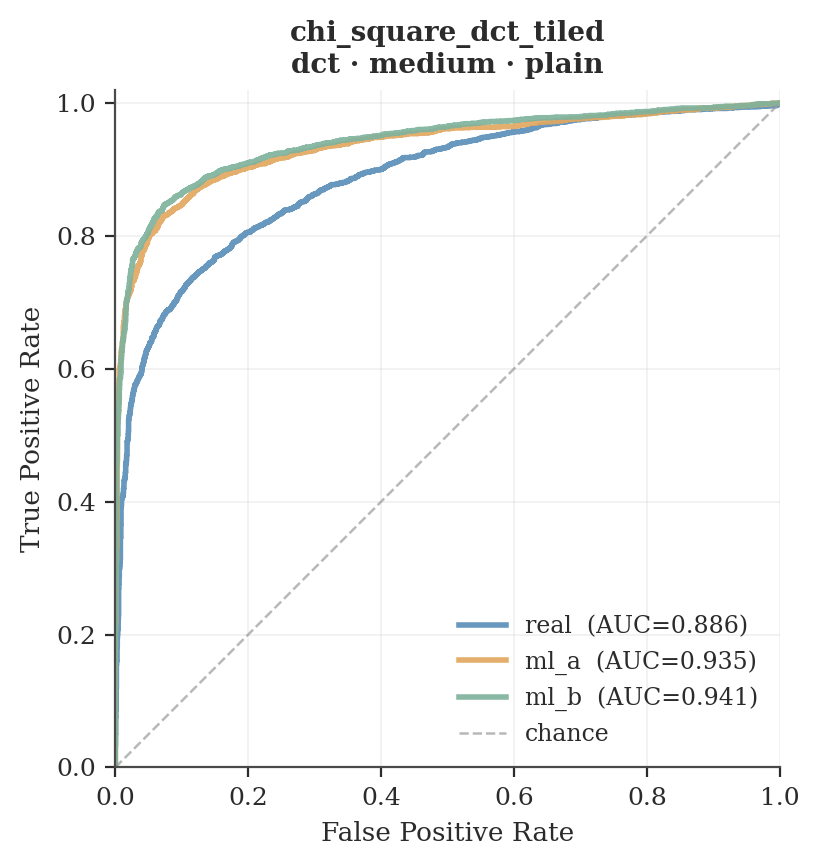
\includegraphics[width=0.86\linewidth]{figures/roc_chi_dct_tiled_med.png}
\caption{ROC curves for $\chi^2$-DCT-tiled at DCT/medium/plain ($N\!=\!3{,}000$). The per-source ordering real (AUC=0.886) $<$ SDXL (0.935) $<$ FLUX (0.941) is consistent with RQ1. The global $\chi^2$-DCT detector on the same data reaches only AUC=0.778, well below the tiled variant.}
\label{fig:tiled}
\end{figure}

\begin{table}[t]
\centering\small
\caption{$\chi^2$-DCT-tiled vs.\ global $\chi^2$-DCT, per (source, payload). Each cell is the per-stratum ROC~AUC; the tiled variant beats the global detector in every cell.}
\label{tab:tiled}
\setlength{\tabcolsep}{4pt}\renewcommand{\arraystretch}{1.1}
\begin{tabular}{@{}l c c c c c c@{}}
\toprule
& \multicolumn{3}{c}{\textbf{$\chi^2$-DCT (global)}} & \multicolumn{3}{c}{\textbf{$\chi^2$-DCT-tiled (ours)}} \\
\cmidrule(lr){2-4}\cmidrule(lr){5-7}
\textbf{Payload} & real & ml\_a & ml\_b & real & ml\_a & ml\_b \\
\midrule
low    & 0.581 & 0.620 & 0.605 & 0.635 & 0.703 & 0.724 \\
medium & 0.727 & 0.806 & 0.775 & 0.886 & 0.936 & 0.941 \\
high   & 0.893 & 0.960 & 0.935 & 0.993 & 0.997 & 0.998 \\
\bottomrule
\end{tabular}
\end{table}

\paragraph{Why does tiling help?} DCT statistics are not spatially uniform across either photographic or diffusion carriers. Textured regions and smooth regions produce very different per-block pairs-of-values histograms. The global detector mixes all blocks into one histogram, which has two effects on the test statistic: (1)~the central-limit averaging hides any localised stego signal, and (2)~the carrier's natural inter-region heterogeneity inflates the cover-side $\chi^2$ noise floor. Tiling separates these regions before applying the test, and max-pooling exposes the tile with the strongest stego-like evidence. The mechanism is the same as Westfeld and Pfitzmann's original sliding-window suggestion~\cite{westfeld1999chi} for detecting \emph{sequential} embedding, but our tiles are coarser and disjoint, which keeps tile-level $\chi^2$ counts large enough to be stable.

\paragraph{Literature support.} Local chi-square variants appear in several places. Westfeld and Pfitzmann themselves discuss a sliding-window form for sequential payloads~\cite{westfeld1999chi}; Provos's outguess paper~\cite{provos2001outguess} notes that the global PoV test loses power as embedding becomes more local; the broader steganalysis literature on \emph{block-wise} or \emph{regional} features (e.g.\ rich-model and DCTR-style approaches~\cite{fridrich2012srm,holub2015dctr}) is essentially built on the same insight at a finer granularity. The tile-local Westfeld $\chi^2$ as we implement it -- a coarse $2\!\times\!2$ disjoint partition with max-pooling, returning the underflow-free $-\chi^2/df$ score -- is a simple and, to our knowledge, under-tested combination of those ingredients.

\paragraph{Caveats and recommended extensions.} Three concerns warrant follow-up:
\begin{enumerate}
\item \textbf{Max-pooling raises false-positive risk.} The detector's score on a cover image is the noisiest of $T^2$ chi-square samples, which can be larger than the global $\chi^2$ on the same image. We control for this in the comparison framework via paired AUC (the same covers and stegos go through both detectors), but a deployed setting would need explicit recalibration against natural-image false-positive rates.
\item \textbf{Tile-size dependence is untested.} We did not sweep $T$. A formal validation should compare $T\!\in\!\{1,2,3,4,6,8\}$ on BOSSBase~\cite{bas2011boss} to check that the choice is not over-fit to our caption-matched dataset.
\item \textbf{Independence from other detectors.} On ML carriers the tile-local detector is the only DCT-branch detector with a practical-significance signal at low payload (Section~\ref{sec:rq1}). It is plausible that the diffusion VAE decoder produces uneven smooth/textured patches that the global detector averages away but the tiled detector locks onto.
\end{enumerate}

We \textbf{recommend two extensions} to validate the finding:
\textit{(a)}~a $T$-sweep on a known steganalysis benchmark (BOSSBase) to triangulate the optimal tile size and rule out over-fitting to our dataset;
\textit{(b)}~a PoV-histogram-variance measurement across tile regions on cover-only data, which would directly verify the heterogeneity hypothesis underlying the gain. Both are inexpensive ($\sim$1 day each) on the existing pipeline.

% ----------------------------------------------------------------
\subsection{Secondary -- The $\chi^2$-Spatial Reversal}
\label{sec:chi2spatial}
% ----------------------------------------------------------------

The single detector that reverses the RQ1 direction is the spatial Westfeld $\chi^2$. At medium and high payload, real photographs are easier to attack than diffusion-generated carriers by 0.027--0.034~AUC, both Holm-significant. The reversal is robust to the $3\!\times\!$ sample size and persists across both SDXL and FLUX.

\paragraph{Mechanism -- direct test.} The Westfeld $\chi^2$ test asks how far the cover's $(2k,\,2k\!+\!1)$ pixel-bit pair counts deviate from equality. To probe the mechanism we ran a falsifying cover-only test: on all 9{,}000 cover images we computed the PoV imbalance
\begin{equation}
S(c) = \sum_{k=0}^{127} |n_{2k}(c) - n_{2k+1}(c)|
\label{eq:pov-imbalance}
\end{equation}
\noindent and the cover-side chi-square score (Figure~\ref{fig:pov}, Appendix~\ref{app:pov}).

The result \emph{falsifies} the naive ``smoother diffusion outputs $\Rightarrow$ lower cover-side $\chi^2_\text{stat}$'' story. The data show the opposite: ML covers have \emph{slightly higher} PoV imbalance than real photographs (medians: real 9{,}698, ml\_a 10{,}272, ml\_b 11{,}649; paired Wilcoxon $p\!<\!10^{-9}$ both directions). The cover-side chi-square score is also more negative (i.e.\ more imbalanced) on ML carriers (medians: real $-4.03$, ml\_a $-4.93$, ml\_b $-6.27$). Diffusion outputs are not more balanced in this sense.

\paragraph{Mechanism -- corrected.} What \emph{does} reverse the AUC is the cover-side score \emph{variance}, not the mean. Cover-side $\chi^2$-spatial score standard deviations are 37.5 (real), 54.4 (ml\_a), 43.0 (ml\_b). At high payload the median cover$\to$stego score shift is in fact \textbf{larger} on ml\_b ($+2.97$) than on real ($+1.95$), but the cover distribution on ML carriers is so much wider that the Cohen's $d$ of cover-vs-stego separation drops from $d\!=\!0.26$ (real) to $d\!=\!0.21$ (ml\_a) and $d\!=\!0.22$ (ml\_b). Interpretation: diffusion outputs have a more \emph{heterogeneous} histogram distribution -- some images are very flat, others very textured -- producing a wider cover-side score distribution that overlaps more with the stego-side distribution, dropping AUC.

\begin{figure}[t]
\centering
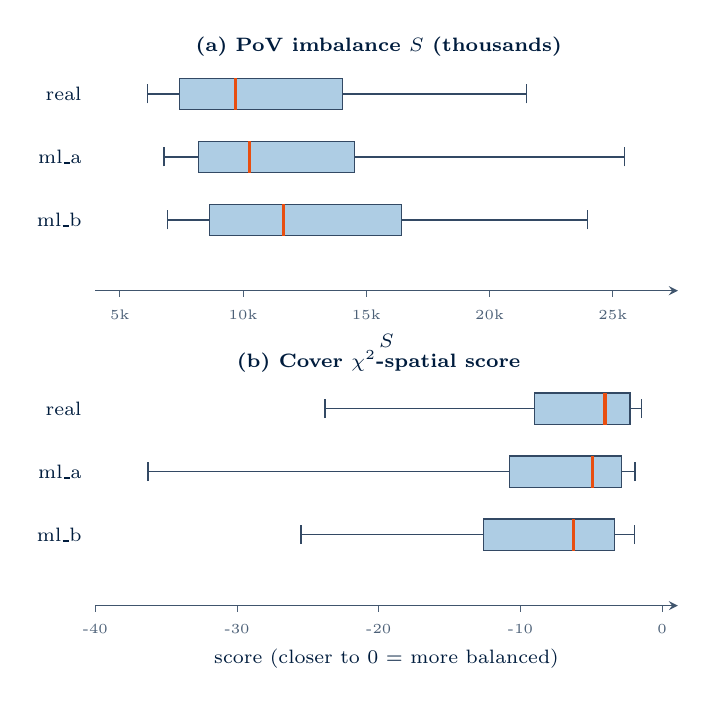
\begin{tikzpicture}[
  whisker/.style={line width=0.5pt, draw=umdark!80},
  box/.style={draw=umdark!80, fill=umlight!45, line width=0.4pt},
  medline/.style={line width=1.2pt, draw=umorange},
  axis/.style={->, >=stealth, umdark!75, line width=0.45pt},
]
% ---------- Panel A: PoV imbalance S (working in kilo-units: divide by 1000 first) ----------
\begin{scope}[shift={(0,0)}]
\node[font=\scriptsize\bfseries\color{umdark}] at (3.6,3.0) {(a) PoV imbalance $S$ (thousands)};
% x-axis: S/1000 in [4, 27], width 7.2 cm, multiplier = 7.2/23 = 0.313
\draw[axis] (0,-0.1) -- (7.4,-0.1);
\foreach \v/\lbl in {5/5k, 10/10k, 15/15k, 20/20k, 25/25k} {
  \pgfmathsetmacro{\x}{(\v-4)*0.313}
  \draw[umdark!70, line width=0.3pt] (\x,-0.1) -- (\x,-0.18);
  \node[font=\tiny\color{umdark!70}, below=1pt] at (\x,-0.18) {\lbl};
}
\node[font=\scriptsize\color{umdark}, below=10pt] at (3.7,-0.18) {$S$};
% per-source rows (S values in thousands)
\foreach \name/\yc/\pa/\qa/\meda/\qb/\pb in {%
  {real}/2.4/6.13/7.42/9.70/14.05/21.49,
  {ml\_a}/1.6/6.79/8.18/10.27/14.52/25.48,
  {ml\_b}/0.8/6.93/8.64/11.65/16.42/23.97%
} {
  \pgfmathsetmacro{\xpa}{(\pa-4)*0.313}
  \pgfmathsetmacro{\xqa}{(\qa-4)*0.313}
  \pgfmathsetmacro{\xmed}{(\meda-4)*0.313}
  \pgfmathsetmacro{\xqb}{(\qb-4)*0.313}
  \pgfmathsetmacro{\xpb}{(\pb-4)*0.313}
  \draw[whisker] (\xpa,\yc) -- (\xpb,\yc);
  \draw[whisker] (\xpa,\yc-0.12) -- (\xpa,\yc+0.12);
  \draw[whisker] (\xpb,\yc-0.12) -- (\xpb,\yc+0.12);
  \draw[box] (\xqa,\yc-0.20) rectangle (\xqb,\yc+0.20);
  \draw[medline] (\xmed,\yc-0.20) -- (\xmed,\yc+0.20);
  \node[font=\scriptsize\color{umdark}, anchor=east] at (-0.05,\yc) {\name};
}
\end{scope}

% ---------- Panel B: cover chi-square score ----------
\begin{scope}[shift={(0,-4.0)}]
\node[font=\scriptsize\bfseries\color{umdark}] at (3.6,3.0) {(b) Cover $\chi^2$-spatial score};
% x-axis: score in [-40, 0], width 7.2 cm, multiplier 7.2/40 = 0.18
\draw[axis] (0,-0.1) -- (7.4,-0.1);
\foreach \v in {-40,-30,-20,-10,0} {
  \pgfmathsetmacro{\x}{(\v+40)*0.18}
  \draw[umdark!70, line width=0.3pt] (\x,-0.1) -- (\x,-0.18);
  \node[font=\tiny\color{umdark!70}, below=1pt] at (\x,-0.18) {\v};
}
\node[font=\scriptsize\color{umdark}, below=10pt] at (3.7,-0.18) {score (closer to 0 = more balanced)};
\foreach \name/\yc/\pa/\qa/\meda/\qb/\pb in {%
  {real}/2.4/-23.78/-9.00/-4.03/-2.27/-1.47,
  {ml\_a}/1.6/-36.27/-10.75/-4.93/-2.87/-1.91,
  {ml\_b}/0.8/-25.48/-12.58/-6.27/-3.36/-1.96%
} {
  \pgfmathsetmacro{\xpa}{(\pa+40)*0.18}
  \pgfmathsetmacro{\xqa}{(\qa+40)*0.18}
  \pgfmathsetmacro{\xmed}{(\meda+40)*0.18}
  \pgfmathsetmacro{\xqb}{(\qb+40)*0.18}
  \pgfmathsetmacro{\xpb}{(\pb+40)*0.18}
  \draw[whisker] (\xpa,\yc) -- (\xpb,\yc);
  \draw[whisker] (\xpa,\yc-0.12) -- (\xpa,\yc+0.12);
  \draw[whisker] (\xpb,\yc-0.12) -- (\xpb,\yc+0.12);
  \draw[box] (\xqa,\yc-0.20) rectangle (\xqb,\yc+0.20);
  \draw[medline] (\xmed,\yc-0.20) -- (\xmed,\yc+0.20);
  \node[font=\scriptsize\color{umdark}, anchor=east] at (-0.05,\yc) {\name};
}
\end{scope}
\end{tikzpicture}
\caption{Cover-only diagnostic for the $\chi^2$-spatial reversal ($n\!=\!3{,}000$ per source). Box = Q1--Q3, whisker = p10--p90, orange line = median. Panel (a): PoV imbalance $S$ from Eq.~\ref{eq:pov-imbalance}; the naive hypothesis predicted ML\,$<$\,real, but real has the \emph{lowest} median (Wilcoxon $p\!<\!10^{-9}$). Panel (b): cover-side $\chi^2$-spatial score; medians track $S$, but the ML distributions are visibly wider (real std 37.5, ml\_a 54.4, ml\_b 43.0). The wider cover-side score distribution is what overwhelms the per-image stego shift and drops the AUC.}
\label{fig:pov}
\end{figure}

\paragraph{Why other detectors are unaffected.} RS analysis and Sample Pairs do not test pair-of-values balance directly; they reason about local pixel-group regularity (RS) or adjacent-pair multiset statistics (SPA). Neither is dominated by the marginal histogram, so the diffusion-decoder heterogeneity does not flip their direction. The DCT-branch detectors operate in frequency space, where diffusion outputs have if anything \emph{more} histogram structure than photographs (due to the JPEG re-encode step), and there the ML-easier direction holds with the largest practical-significance effects.

\paragraph{Where the reversal lives.} Crucially, the reversal is a \emph{full-AUC} artefact. Under the partial-AUC view at FPR\,$\leq\!0.10$, all three $\chi^2$-spatial strata have $|\Delta_\text{pAUC}|\!\leq\!0.007$ and none reaches Holm significance. The diffusion-flatness fingerprint lives in the high-FPR tail of the ROC curve, the region where a real steganalyst would never operate. In other words: the reversal is mathematically real but operationally negligible. We report it as a mechanistic observation rather than as a counter-example to RQ1's main direction.

\paragraph{Generalisation.} A natural follow-up is to extend the carrier-source set to additional diffusion families (Stable Diffusion~3, FLUX.1-dev, Midjourney) to check that the cover-side variance-inflation effect is a general property of latent-diffusion decoders rather than an SDXL-or-FLUX idiosyncrasy. We leave this to future work.

% ============================================================
\section{Limitations}
\label{sec:limitations}
% ============================================================

\paragraph{Pre-registered deviations.} Two changes from the proposal are acknowledged: \textit{(i)}~ML-B was migrated from PixArt-$\alpha$~\cite{pixart2023} to FLUX.1-schnell~\cite{flux2024} because the former lost HF Inference API support during Phase~2; \textit{(ii)}~payload fill rates were lowered from $\{0.25,0.50,0.75\}$ to $\{0.05,0.15,0.30\}$~bpp to avoid detector saturation. Both changes are documented in the run config and the slides. The first does not affect the RQ design (still two diffusion families with caption-matched outputs); the second strengthens the comparison by placing the experiment in a more operationally realistic regime.

\paragraph{Scope bounds.} Two generator families only; we cannot disentangle architecture from training data in RQ2. Grayscale only; colour information is intentionally removed for closer comparability with BOSSBase~\cite{bas2011boss} and the published detectors, but a colour study would be informative. The \emph{primary} (pre-registered) Bonferroni--Holm family contains only the six classical training-free detectors; the learned baselines (SRNet and DCTR) are reported with a separate Bonferroni--Holm correction over their own 6-stratum family in Section~\ref{sec:learnedxval} so the pre-registered correction in Table~\ref{tab:verdicts} is preserved exactly. RQ4 pools an asymmetric set (three spatial vs.\ three frequency detectors after adding the tile-local variant); the branch contrast accounts for this in its inverse-variance weighting.

\paragraph{Learned-detector caveats.} Three caveats accompany the supplementary learned-detector analysis. \textit{(i)} A single training-set random seed is used; we do not report multi-seed variability of the learned-AUC estimates. \textit{(ii)} The DCTR feature extractor uses the 8{,}000-dim variant of Holub \& Fridrich~\cite{holub2015dctr} interpreted as 64 modes $\times$ 25 phases (5$\times$5 alignment subset) $\times$ 5 truncated bins; the exact phase decomposition that yields the paper's headline 8{,}000 count is somewhat ambiguous from the paper text alone, and our interpretation is one of several defensible reconstructions. \textit{(iii)} SRNet is trained on caption-matched data, not on BOSSBase; this is the academically preferable choice for our cover-source-mismatch-aware design, but it makes our AUC numbers not directly comparable to literature SRNet figures on BOSSBase.

\paragraph{Engineering caveats.} The analysis pipeline's ROC computation is implemented as a pure-Python $O(N^2)$ scan over per-threshold confusion-matrix updates ([src/evaluation/metrics.py]); for 648{,}000 predictions this took roughly six wall-clock hours on a single CPU. A vectorised \texttt{sklearn.metrics.roc\_curve} equivalent would complete the same work in seconds. The result is correct; the cost is excessive. This is flagged as a Phase~3 cleanup item.

% ============================================================
\section{Conclusion and Future Work}
\label{sec:conclusion}
% ============================================================

We ran a caption-matched 6-detector $\times$ 2-method $\times$ 3-payload $\times$ 2-encryption factorial on 3{,}000 caption groups (108{,}000 stego images, 648{,}000 classical-detector predictions) to ask whether carrier source -- real photograph vs.\ diffusion-generated synthetic image -- changes the detectability of LSB-style steganography under matched embedding. Five of six training-free detectors agree that diffusion carriers are slightly easier to attack than photographs, with the gap concentrated at low payload (RQ1, RQ3); the two diffusion models we tested are interchangeable at the detector level (RQ2); the source effect is statistically similar across spatial and frequency embedding branches once pooled (RQ4); and AES-256-CBC encryption of the payload has no measurable detectability effect (RQ5). The partial-AUC analysis at FPR\,$\leq\!0.10$ amplifies every RQ1 effect by 3--7$\times$ and elevates the verdict from mixed to supported. A cross-validation on two methodologically orthogonal learned baselines (SRNet for the spatial branch, DCTR for the frequency branch), trained on a disjoint 3{,}000-caption corpus, corroborates RQ2, RQ4 and RQ5 directly, refines RQ3 to roughly half the classical magnitude with the same monotone direction, and clarifies RQ1: DCTR (a hand-crafted frequency feature set scored by an LDA ensemble) reproduces the classical real-harder pattern at $\Delta_\text{AUC}\!\approx\!-0.030$ within its branch, while SRNet (a deep spatial CNN, saturated at AUC $\geq 0.997$) abstracts the source signal away -- an outcome the V2a real-only-training ablation disentangles into either architectural source-invariance or a balanced-training artefact (\S\ref{sec:v2a}).

Two secondary contributions warrant follow-up:
\begin{itemize}
\item the \textbf{tile-local Westfeld $\chi^2$ variant}, which out-performs the global PoV detector by a wide margin on our data and is a natural candidate for a stand-alone validation against established steganalysis benchmarks;
\item the mechanistic account of the \textbf{$\chi^2$-spatial reversal} as a high-FPR diffusion-decoder fingerprint, which the pAUC analysis confirms is operationally negligible.
\end{itemize}

Operationally, our conclusion is that a steganalyst deploying classical detectors against diffusion-generated carriers should expect to do at least as well as against ordinary photographs, and substantially better at low embedding rates in the operationally screened FPR regime.

\paragraph{Future work.} Two concrete one-day extensions reuse the existing pipeline: a \textbf{lower-payload tier} (0.01 / 0.02~bpp) via \texttt{rerun\_with\_existing\_covers.py}, expected to widen the source gap on RS and sample-pairs; and a \textbf{tile-size sweep} for $\chi^2$-DCT-tiled on BOSSBase~\cite{bas2011boss}, $T\!\in\!\{1,2,3,4,6,8\}$, to validate the tile-local detector against the field's reference dataset. The PoV-imbalance measurement (Equation~\ref{eq:pov-imbalance}) was originally planned as future work but is now reported inline (Section~\ref{sec:chi2spatial}); it falsified the naive smoothness hypothesis and surfaced a cover-side-variance mechanism that future work could probe further. The learned-baseline extension flagged in earlier drafts (``adding an SRNet-style learned baseline to close the most prominent reviewer concern'') is now fully integrated as the cross-validation analysis of Section~\ref{sec:learnedxval}, including a V2a real-only-training ablation that addresses the architectural-vs-balanced-training ambiguity exposed by SRNet's near-saturation. Medium-effort extensions include a JPEG-quality sweep, a colour-mode study (YCbCr-Y), a multi-seed sensitivity analysis of the learned-detector AUCs, and applying SRNet to the DCT branch (decompressed JPEG inputs) to give a same-architecture spatial-vs-frequency learned comparison.

% ============================================================
\clearpage
\renewcommand{\refname}{References}
% ============================================================

\begin{thebibliography}{30}\small

\bibitem{petitcolas1999}
F.~A.~P.~Petitcolas, R.~J.~Anderson, and M.~G.~Kuhn,
``Information hiding: a survey,''
\textit{Proc.\ IEEE}, vol.~87, no.~7, pp.~1062--1078, 1999.

\bibitem{cheddad2010}
A.~Cheddad, J.~Condell, K.~Curran, and P.~McKevitt,
``Digital image steganography: Survey and analysis of current methods,''
\textit{Signal Process.}, vol.~90, no.~3, pp.~727--752, 2010.

\bibitem{hussain2018}
M.~Hussain, A.~W.~A.~Wahab, Y.~I.~B.~Idris, A.~T.~S.~Ho, and K.~H.~Jung,
``Image steganography in spatial domain: A survey,''
\textit{Signal Process.: Image Commun.}, vol.~65, pp.~46--66, 2018.

\bibitem{westfeld1999chi}
A.~Westfeld and A.~Pfitzmann,
``Attacks on steganographic systems,''
in \textit{Proc.\ 3rd Int.\ Workshop Information Hiding}, LNCS 1768, pp.~61--76, 1999.

\bibitem{fridrich2001lsb}
J.~Fridrich, M.~Goljan, and R.~Du,
``Reliable detection of LSB steganography in color and grayscale images,''
\textit{IEEE Multimedia}, vol.~8, no.~4, pp.~22--28, 2001.

\bibitem{dumitrescu2003sp}
S.~Dumitrescu, X.~Wu, and Z.~Wang,
``Detection of LSB steganography via sample pair analysis,''
\textit{IEEE Trans.\ Signal Process.}, vol.~51, no.~7, pp.~1995--2007, 2003.

\bibitem{fridrich2003calib}
J.~Fridrich, M.~Goljan, and D.~Hogea,
``New methodology for breaking steganographic techniques for JPEGs,''
in \textit{Proc.\ SPIE Electronic Imaging}, vol.~5020, pp.~143--155, 2003.

\bibitem{provos2001outguess}
N.~Provos,
``Defending against statistical steganalysis,''
in \textit{Proc.\ 10th USENIX Security Symposium}, pp.~323--335, 2001.

\bibitem{fridrich2012srm}
J.~Fridrich and J.~Kodovsk\'{y},
``Rich models for steganalysis of digital images,''
\textit{IEEE Trans.\ Inf.\ Forensics Security}, vol.~7, no.~3, pp.~868--882, 2012.

\bibitem{holub2015dctr}
V.~Holub and J.~Fridrich,
``Low-complexity features for JPEG steganalysis using undecimated DCT,''
\textit{IEEE Trans.\ Inf.\ Forensics Security}, vol.~10, no.~2, pp.~219--228, 2015.

\bibitem{boroumand2019srnet}
M.~Boroumand, M.~Chen, and J.~Fridrich,
``Deep residual network for steganalysis of digital images,''
\textit{IEEE Trans.\ Inf.\ Forensics Security}, vol.~14, no.~5, pp.~1181--1193, 2019.

\bibitem{delong1988}
E.~R.~DeLong, D.~M.~DeLong, and D.~L.~Clarke-Pearson,
``Comparing the areas under two or more correlated receiver operating characteristic curves: a nonparametric approach,''
\textit{Biometrics}, vol.~44, no.~3, pp.~837--845, 1988.

\bibitem{mcclish1989}
D.~K.~McClish,
``Analyzing a portion of the ROC curve,''
\textit{Medical Decision Making}, vol.~9, no.~3, pp.~190--195, 1989.

\bibitem{giboulot2020csm}
Q.~Giboulot, R.~Cogranne, D.~Borghys, and P.~Bas,
``Effects and solutions of cover-source mismatch in image steganalysis,''
\textit{Signal Process.: Image Commun.}, vol.~86, art.~115888, 2020.

\bibitem{mallet2024csm}
A.~Mallet, M.~Bene\v{s}, and R.~Cogranne,
``Cover-source mismatch in steganalysis: Systematic review,''
\textit{EURASIP J.\ Inf.\ Security}, vol.~2024, art.~26, 2024.

\bibitem{mereur2024deepfake}
A.~M\'{e}reur, A.~Mallet, and R.~Cogranne,
``Are deepfakes a game-changer in digital images steganography leveraging the cover-source mismatch?''
in \textit{Proc.\ 19th Int.\ Conf.\ Availability, Reliability and Security (ARES)}, 9~pages, 2024.

\bibitem{gao2022ai}
K.~Gao, C.-C.~Chang, J.-H.~Horng, and I.~Echizen,
``Steganographic secret sharing via AI-generated photorealistic images,''
\textit{EURASIP J.\ Wireless Commun.\ Netw.}, vol.~2022, art.~119, 2022.

\bibitem{corvi2023diffusion}
R.~Corvi, D.~Cozzolino, G.~Zingarini, G.~Poggi, K.~Nagano, and L.~Verdoliva,
``On the detection of synthetic images generated by diffusion models,''
in \textit{Proc.\ IEEE ICASSP}, pp.~1--5, 2023.

\bibitem{hou2021gan}
J.~Hou, S.~Marra, F.~Marra, M.~Iuliani, and L.~Verdoliva,
``Survey of GAN-generated image detection methods,''
\textit{arXiv:2102.12158}, 2021.

\bibitem{rossler2019fake}
A.~R\"ossler, D.~Cozzolino, L.~Verdoliva, C.~Riess, J.~Thies, and M.~Nie{\ss}ner,
``FaceForensics++: Learning to detect manipulated facial images,''
in \textit{Proc.\ ICCV}, pp.~1--11, 2019.

\bibitem{sdxl2023}
D.~Podell et al.,
``SDXL: Improving latent diffusion models for high-resolution image synthesis,''
in \textit{Proc.\ Int.\ Conf.\ Learning Representations (ICLR)}, 2024.
arXiv:2307.01952.

\bibitem{pixart2023}
J.~Chen et al.,
``PixArt-$\alpha$: Fast training of diffusion transformer for photorealistic text-to-image synthesis,''
in \textit{Proc.\ Int.\ Conf.\ Learning Representations (ICLR)}, 2024.

\bibitem{flux2024}
Black~Forest~Labs,
``FLUX.1-schnell,''
2024.
\url{https://huggingface.co/black-forest-labs/FLUX.1-schnell}.

\bibitem{coco2014}
T.-Y.~Lin et al.,
``Microsoft COCO: Common objects in context,''
in \textit{Proc.\ ECCV}, LNCS 8693, pp.~740--755, 2014.

\bibitem{flickr30k2014}
P.~Young, A.~Lai, M.~Hodosh, and J.~Hockenmaier,
``From image descriptions to visual denotations: New similarity metrics for semantic inference over event descriptions,''
\textit{Trans.\ Assoc.\ Comput.\ Linguist.}, vol.~2, pp.~67--78, 2014.

\bibitem{bas2011boss}
P.~Bas, T.~Filler, and T.~Pevn\'{y},
``Break our steganographic system: The ins and outs of organizing BOSS,''
in \textit{Proc.\ 13th Int.\ Conf.\ Information Hiding}, LNCS 6958, pp.~59--70, 2011.

\bibitem{zhang2011fsim}
L.~Zhang, L.~Zhang, X.~Mou, and D.~Zhang,
``FSIM: A feature similarity index for image quality assessment,''
\textit{IEEE Trans.\ Image Process.}, vol.~20, no.~8, pp.~2378--2386, 2011.

\bibitem{mittal2012brisque}
A.~Mittal, A.~K.~Moorthy, and A.~C.~Bovik,
``No-reference image quality assessment in the spatial domain,''
\textit{IEEE Trans.\ Image Process.}, vol.~21, no.~12, pp.~4695--4708, 2012.

\end{thebibliography}

% ============================================================
\onecolumn
\appendix
\section*{Appendix}
\addcontentsline{toc}{section}{Appendix}
\renewcommand{\thesection}{\Alph{section}}
\setcounter{section}{0}

\section{Run Configuration}
\label{app:config}
The active configuration of the $N\!=\!3{,}000$ confirmatory run, as stored in \texttt{runs/prototype\_full\_20260513\_005357\_p8765/.meta.json}:
\begin{lstlisting}[language=,basicstyle=\ttfamily\small,frame=single,framerule=0pt,backgroundcolor=\color{codebg}]
{
  "profile":             "prototype_full",
  "engine":              "inference_api",
  "n_groups":            3000,
  "active_methods":      ["lsb", "dct"],
  "active_payload_levels": ["low", "medium", "high"],
  "payload_fill_rates":  {"low": 0.05,
                          "medium": 0.15,
                          "high": 0.30},
  "active_encryption":   ["plain", "encrypted"],
  "active_detectors":    ["rs",
                          "chi_square_spatial",
                          "sample_pairs",
                          "chi_square_dct",
                          "chi_square_dct_tiled",
                          "calibration_chi_square"],
  "jpeg_quality":        95,
  "payload_mode":        "random"
}
\end{lstlisting}

\section{Per-stratum DeLong Contrasts (RQ1)}
\label{app:rq1-delong}
Table~\ref{tab:appendix-rq1} gives the full 18-stratum DeLong table for RQ1, including per-source AUCs, the paired $\Delta_\text{AUC}$, its 95\% CI from the DeLong variance estimator, the z-statistic, and both the raw p-value and the Holm-corrected p-value (family size 18). Sixteen of eighteen strata are Holm-significant; the only insignificant strata are calibration $\chi^2$/dct/low ($p_\text{Holm}\!=\!0.21$) and $\chi^2$-spatial/lsb/low ($p_\text{Holm}\!=\!0.21$).

\begin{table*}[h]
\centering\footnotesize
\caption{RQ1 -- per-stratum paired DeLong contrast (real $-$ pooled ML), $N\!=\!3{,}000$.}
\label{tab:appendix-rq1}
\setlength{\tabcolsep}{4pt}\renewcommand{\arraystretch}{1.1}
\begin{tabular}{@{}l l l c c c r r r r r@{}}
\toprule
\textbf{Detector} & \textbf{Mth} & \textbf{Payload} & \textbf{AUC\,real} & \textbf{AUC\,ml\_a} & \textbf{AUC\,ml\_b} & \textbf{$\Delta$} & \textbf{CI\textsubscript{lo}} & \textbf{CI\textsubscript{hi}} & \textbf{$p$} & \textbf{$p_\text{Holm}$} \\
\midrule
cal-$\chi^2$         & DCT & low    & 0.519 & 0.528 & 0.531 & $-0.009$ & $-0.022$ & $+0.003$ & $1.5\!\times\!10^{-1}$ & $2.1\!\times\!10^{-1}$ \\
cal-$\chi^2$         & DCT & med    & 0.550 & 0.577 & 0.580 & $-0.023$ & $-0.036$ & $-0.011$ & $3.0\!\times\!10^{-4}$ & $1.0\!\times\!10^{-3}$ \\
cal-$\chi^2$         & DCT & high   & 0.586 & 0.642 & 0.635 & $-0.045$ & $-0.058$ & $-0.033$ & $5.5\!\times\!10^{-13}$ & $4.4\!\times\!10^{-12}$ \\
$\chi^2$-DCT         & DCT & low    & 0.581 & 0.620 & 0.605 & $-0.025$ & $-0.038$ & $-0.013$ & $6.0\!\times\!10^{-5}$ & $3.0\!\times\!10^{-4}$ \\
$\chi^2$-DCT         & DCT & med    & 0.727 & 0.806 & 0.775 & $-0.051$ & $-0.062$ & $-0.041$ & $<\!10^{-15}$           & $<\!10^{-15}$ \\
$\chi^2$-DCT         & DCT & high   & 0.893 & 0.960 & 0.935 & $-0.048$ & $-0.054$ & $-0.041$ & $<\!10^{-15}$           & $<\!10^{-15}$ \\
$\chi^2$-DCT-tiled   & DCT & low    & 0.635 & 0.703 & 0.724 & $-0.060$ & $-0.072$ & $-0.048$ & $<\!10^{-15}$           & $<\!10^{-15}$ \\
$\chi^2$-DCT-tiled   & DCT & med    & 0.886 & 0.936 & 0.941 & $-0.039$ & $-0.046$ & $-0.033$ & $<\!10^{-15}$           & $<\!10^{-15}$ \\
$\chi^2$-DCT-tiled   & DCT & high   & 0.993 & 0.997 & 0.998 & $-0.003$ & $-0.005$ & $-0.001$ & $2.5\!\times\!10^{-4}$ & $1.0\!\times\!10^{-3}$ \\
$\chi^2$-spatial     & LSB & low    & 0.541 & 0.530 & 0.533 & $+0.010$ & $-0.002$ & $+0.023$ & $1.0\!\times\!10^{-1}$ & $2.1\!\times\!10^{-1}$ \\
$\chi^2$-spatial     & LSB & med    & 0.608 & 0.574 & 0.590 & $+0.027$ & $+0.015$ & $+0.040$ & $1.4\!\times\!10^{-5}$ & $8.5\!\times\!10^{-5}$ \\
$\chi^2$-spatial     & LSB & high   & 0.694 & 0.646 & 0.675 & $+0.034$ & $+0.023$ & $+0.046$ & $5.8\!\times\!10^{-9}$ & $4.0\!\times\!10^{-8}$ \\
RS                   & LSB & low    & 0.856 & 0.941 & 0.952 & $-0.090$ & $-0.098$ & $-0.083$ & $<\!10^{-15}$           & $<\!10^{-15}$ \\
RS                   & LSB & med    & 0.962 & 0.992 & 0.994 & $-0.030$ & $-0.034$ & $-0.027$ & $<\!10^{-15}$           & $<\!10^{-15}$ \\
RS                   & LSB & high   & 0.989 & 0.998 & 0.999 & $-0.010$ & $-0.011$ & $-0.008$ & $<\!10^{-15}$           & $<\!10^{-15}$ \\
sample-pairs         & LSB & low    & 0.883 & 0.974 & 0.971 & $-0.089$ & $-0.096$ & $-0.082$ & $<\!10^{-15}$           & $<\!10^{-15}$ \\
sample-pairs         & LSB & med    & 0.975 & 0.998 & 0.995 & $-0.022$ & $-0.025$ & $-0.019$ & $<\!10^{-15}$           & $<\!10^{-15}$ \\
sample-pairs         & LSB & high   & 0.993 & 1.000 & 0.999 & $-0.007$ & $-0.008$ & $-0.005$ & $3.6\!\times\!10^{-15}$ & $3.2\!\times\!10^{-14}$ \\
\bottomrule
\end{tabular}
\end{table*}

\section{Per-stratum DeLong Contrasts (RQ2)}
\label{app:rq2-delong}
Table~\ref{tab:appendix-rq2} gives the analogous 18-stratum DeLong table for RQ2 (SDXL $-$ FLUX). Seven of eighteen strata are Holm-significant; none clears the pre-registered $\delta_\text{min}\!=\!0.05$ gate. The largest magnitudes are $\chi^2$-DCT/dct/med ($+0.031$) and $\chi^2$-spatial/lsb/high ($-0.029$), both Holm-significant and both clearing the supplementary $\delta_\text{min}\!=\!0.025$.

\begin{table*}[h]
\centering\footnotesize
\caption{RQ2 -- per-stratum paired DeLong contrast (SDXL $-$ FLUX), $N\!=\!3{,}000$.}
\label{tab:appendix-rq2}
\setlength{\tabcolsep}{4pt}\renewcommand{\arraystretch}{1.1}
\begin{tabular}{@{}l l l c c r r r r r@{}}
\toprule
\textbf{Detector} & \textbf{Mth} & \textbf{Payload} & \textbf{AUC\,SDXL} & \textbf{AUC\,FLUX} & \textbf{$\Delta$} & \textbf{CI\textsubscript{lo}} & \textbf{CI\textsubscript{hi}} & \textbf{$p$} & \textbf{$p_\text{Holm}$} \\
\midrule
cal-$\chi^2$         & DCT & low    & 0.528 & 0.531 & $-0.003$ & $-0.018$ & $+0.011$ & $0.68$  & $1.00$ \\
cal-$\chi^2$         & DCT & med    & 0.577 & 0.580 & $-0.002$ & $-0.016$ & $+0.012$ & $0.77$  & $1.00$ \\
cal-$\chi^2$         & DCT & high   & 0.642 & 0.635 & $+0.006$ & $-0.008$ & $+0.020$ & $0.38$  & $1.00$ \\
$\chi^2$-DCT         & DCT & low    & 0.620 & 0.605 & $+0.015$ & $+0.001$ & $+0.029$ & $4.2\!\times\!10^{-2}$  & $4.2\!\times\!10^{-1}$ \\
$\chi^2$-DCT         & DCT & med    & 0.806 & 0.775 & $+0.031$ & $+0.020$ & $+0.043$ & $5.7\!\times\!10^{-8}$  & $9.8\!\times\!10^{-7}$ \\
$\chi^2$-DCT         & DCT & high   & 0.960 & 0.935 & $+0.025$ & $+0.020$ & $+0.030$ & $<\!10^{-15}$            & $<\!10^{-15}$ \\
$\chi^2$-DCT-tiled   & DCT & low    & 0.703 & 0.724 & $-0.021$ & $-0.034$ & $-0.008$ & $1.6\!\times\!10^{-3}$  & $1.9\!\times\!10^{-2}$ \\
$\chi^2$-DCT-tiled   & DCT & med    & 0.936 & 0.941 & $-0.005$ & $-0.011$ & $+0.001$ & $1.1\!\times\!10^{-1}$  & $8.5\!\times\!10^{-1}$ \\
$\chi^2$-DCT-tiled   & DCT & high   & 0.997 & 0.998 & $-0.001$ & $-0.002$ & $+0.000$ & $1.3\!\times\!10^{-1}$  & $9.2\!\times\!10^{-1}$ \\
$\chi^2$-spatial     & LSB & low    & 0.530 & 0.533 & $-0.003$ & $-0.018$ & $+0.012$ & $0.69$  & $1.00$ \\
$\chi^2$-spatial     & LSB & med    & 0.574 & 0.590 & $-0.016$ & $-0.030$ & $-0.001$ & $3.4\!\times\!10^{-2}$  & $3.7\!\times\!10^{-1}$ \\
$\chi^2$-spatial     & LSB & high   & 0.646 & 0.675 & $-0.029$ & $-0.042$ & $-0.015$ & $3.9\!\times\!10^{-5}$  & $6.3\!\times\!10^{-4}$ \\
RS                   & LSB & low    & 0.941 & 0.952 & $-0.011$ & $-0.017$ & $-0.005$ & $5.4\!\times\!10^{-4}$  & $7.0\!\times\!10^{-3}$ \\
RS                   & LSB & med    & 0.992 & 0.994 & $-0.002$ & $-0.004$ & $+0.000$ & $6.4\!\times\!10^{-2}$  & $5.8\!\times\!10^{-1}$ \\
RS                   & LSB & high   & 0.998 & 0.999 & $-0.000$ & $-0.001$ & $+0.000$ & $2.7\!\times\!10^{-1}$  & $1.00$ \\
sample-pairs         & LSB & low    & 0.974 & 0.971 & $+0.004$ & $-0.001$ & $+0.008$ & $1.4\!\times\!10^{-1}$  & $9.2\!\times\!10^{-1}$ \\
sample-pairs         & LSB & med    & 0.998 & 0.995 & $+0.003$ & $+0.002$ & $+0.005$ & $6.2\!\times\!10^{-5}$  & $9.3\!\times\!10^{-4}$ \\
sample-pairs         & LSB & high   & 1.000 & 0.999 & $+0.001$ & $+0.001$ & $+0.002$ & $4.0\!\times\!10^{-4}$  & $5.6\!\times\!10^{-3}$ \\
\bottomrule
\end{tabular}
\end{table*}

\section{Per-stratum Partial-AUC Contrasts at FPR\,$\leq\!0.10$}
\label{app:pauc-table}
Table~\ref{tab:appendix-pauc} gives the 18-stratum McClish-normalised partial AUC contrasts for RQ1 with bootstrap standard errors (500 resamples per stratum) and Holm-corrected p-values within the 18-test family.

\begin{table}[!htbp]
\centering\footnotesize
\caption{RQ1 -- per-stratum partial AUC contrast at FPR\,$\leq\!0.10$ (real $-$ pooled ML).}
\label{tab:appendix-pauc}
\setlength{\tabcolsep}{4pt}\renewcommand{\arraystretch}{1.1}
\begin{tabular}{@{}l l l r r r@{}}
\toprule
\textbf{Detector} & \textbf{Mth} & \textbf{Payload} & \textbf{$\Delta_\text{pAUC}$} & \textbf{SE} & \textbf{$p_\text{Holm}$} \\
\midrule
cal-$\chi^2$         & DCT & low    & $-0.002$ & $0.003$ & $1.00$ \\
cal-$\chi^2$         & DCT & med    & $-0.004$ & $0.003$ & $0.69$ \\
cal-$\chi^2$         & DCT & high   & $-0.010$ & $0.003$ & $4.9\!\times\!10^{-3}$ \\
$\chi^2$-DCT         & DCT & low    & $-0.002$ & $0.003$ & $1.00$ \\
$\chi^2$-DCT         & DCT & med    & $-0.015$ & $0.005$ & $1.7\!\times\!10^{-2}$ \\
$\chi^2$-DCT         & DCT & high   & $-0.057$ & $0.006$ & $<\!10^{-15}$ \\
$\chi^2$-DCT-tiled   & DCT & low    & $-0.038$ & $0.004$ & $<\!10^{-15}$ \\
$\chi^2$-DCT-tiled   & DCT & med    & $-0.064$ & $0.006$ & $<\!10^{-15}$ \\
$\chi^2$-DCT-tiled   & DCT & high   & $-0.006$ & $0.002$ & $1.1\!\times\!10^{-3}$ \\
$\chi^2$-spatial     & LSB & low    & $+0.001$ & $0.003$ & $1.00$ \\
$\chi^2$-spatial     & LSB & med    & $+0.003$ & $0.003$ & $1.00$ \\
$\chi^2$-spatial     & LSB & high   & $+0.007$ & $0.005$ & $0.72$ \\
RS                   & LSB & low    & $-0.156$ & $0.009$ & $<\!10^{-15}$ \\
RS                   & LSB & med    & $-0.092$ & $0.006$ & $<\!10^{-15}$ \\
RS                   & LSB & high   & $-0.039$ & $0.003$ & $<\!10^{-15}$ \\
sample-pairs         & LSB & low    & $-0.296$ & $0.009$ & $<\!10^{-15}$ \\
sample-pairs         & LSB & med    & $-0.109$ & $0.008$ & $<\!10^{-15}$ \\
sample-pairs         & LSB & high   & $-0.034$ & $0.004$ & $7.1\!\times\!10^{-14}$ \\
\bottomrule
\end{tabular}
\end{table}

\section{Score-Level Paired t-Tests}
\label{app:t-tests}
Table~\ref{tab:appendix-ttest} reports paired Student's t-tests on the \emph{raw detector scores} across the four pre-registered comparisons (3 source contrasts $\times$ 6 detectors $+$ plain vs.\ AES-256-CBC $\times$ 6 detectors $=24$ tests). Holm correction is applied within the 24-test family. Effect sizes are Cohen's $d$ (small $\!=\!0.2$, medium $\!=\!0.5$, large $\!=\!0.8$). The encryption comparisons (top block) all have $|d|\!\leq\!0.029$ and are consistent with the RQ5 null; the carrier-source comparisons show large effects on the strongest detectors (RS, sample-pairs) and the new $\chi^2$-DCT-tiled.

\begin{table}[!htbp]
\centering\footnotesize
\caption{Score-level paired t-tests across all pre-registered comparisons. $n$ is the number of paired score samples per test.}
\label{tab:appendix-ttest}
\setlength{\tabcolsep}{4pt}\renewcommand{\arraystretch}{1.1}
\begin{tabular}{@{}l l c r r r r r@{}}
\toprule
\textbf{Comparison} & \textbf{Detector} & \textbf{$n$} & \textbf{$t$} & \textbf{$p$} & \textbf{$p_\text{Holm}$} & \textbf{Cohen's $d$} & \textbf{Sig.} \\
\midrule
plain vs AES   & cal-$\chi^2$       & 27\,000 & $-0.57$ & $0.57$ & $1.00$ & $-0.003$ & \\
plain vs AES   & $\chi^2$-DCT       & 27\,000 & $-0.77$ & $0.44$ & $1.00$ & $-0.005$ & \\
plain vs AES   & $\chi^2$-DCT-tiled & 27\,000 & $+0.12$ & $0.90$ & $1.00$ & $+0.001$ & \\
plain vs AES   & $\chi^2$-spatial   & 27\,000 & $+4.82$ & $10^{-6}$  & $3.5\!\times\!10^{-5}$ & $+0.029$ & $\checkmark$ \\
plain vs AES   & RS                 & 27\,000 & $+4.16$ & $3.2\!\times\!10^{-5}$ & $7.6\!\times\!10^{-4}$ & $+0.025$ & $\checkmark$ \\
plain vs AES   & sample-pairs       & 27\,000 & $+4.33$ & $1.5\!\times\!10^{-5}$ & $3.6\!\times\!10^{-4}$ & $+0.026$ & $\checkmark$ \\
\midrule
real vs SDXL   & cal-$\chi^2$       & 18\,000 & $+9.66$  & $<\!10^{-15}$ & $<\!10^{-15}$ & $+0.072$ & $\checkmark$ \\
real vs SDXL   & $\chi^2$-DCT       & 18\,000 & $-19.97$ & $<\!10^{-15}$ & $<\!10^{-15}$ & $-0.149$ & $\checkmark$ \\
real vs SDXL   & $\chi^2$-DCT-tiled & 18\,000 & $-22.17$ & $<\!10^{-15}$ & $<\!10^{-15}$ & $-0.165$ & $\checkmark$ \\
real vs SDXL   & $\chi^2$-spatial   & 18\,000 & $+15.77$ & $<\!10^{-15}$ & $<\!10^{-15}$ & $+0.118$ & $\checkmark$ \\
real vs SDXL   & RS                 & 18\,000 & $-51.69$ & $<\!10^{-15}$ & $<\!10^{-15}$ & $-0.385$ & $\checkmark$ \\
real vs SDXL   & sample-pairs       & 18\,000 & $+53.79$ & $<\!10^{-15}$ & $<\!10^{-15}$ & $+0.401$ & $\checkmark$ \\
\midrule
real vs FLUX   & cal-$\chi^2$       & 18\,000 & $-15.52$ & $<\!10^{-15}$ & $<\!10^{-15}$ & $-0.116$ & $\checkmark$ \\
real vs FLUX   & $\chi^2$-DCT       & 18\,000 & $-34.71$ & $<\!10^{-15}$ & $<\!10^{-15}$ & $-0.259$ & $\checkmark$ \\
real vs FLUX   & $\chi^2$-DCT-tiled & 18\,000 & $-48.67$ & $<\!10^{-15}$ & $<\!10^{-15}$ & $-0.363$ & $\checkmark$ \\
real vs FLUX   & $\chi^2$-spatial   & 18\,000 & $+9.14$  & $<\!10^{-15}$ & $<\!10^{-15}$ & $+0.068$ & $\checkmark$ \\
real vs FLUX   & RS                 & 18\,000 & $-71.49$ & $<\!10^{-15}$ & $<\!10^{-15}$ & $-0.533$ & $\checkmark$ \\
real vs FLUX   & sample-pairs       & 18\,000 & $+34.80$ & $<\!10^{-15}$ & $<\!10^{-15}$ & $+0.259$ & $\checkmark$ \\
\midrule
SDXL vs FLUX   & cal-$\chi^2$       & 18\,000 & $-65.19$ & $<\!10^{-15}$ & $<\!10^{-15}$ & $-0.486$ & $\checkmark$ \\
SDXL vs FLUX   & $\chi^2$-DCT       & 18\,000 & $-58.97$ & $<\!10^{-15}$ & $<\!10^{-15}$ & $-0.440$ & $\checkmark$ \\
SDXL vs FLUX   & $\chi^2$-DCT-tiled & 18\,000 & $-70.68$ & $<\!10^{-15}$ & $<\!10^{-15}$ & $-0.527$ & $\checkmark$ \\
SDXL vs FLUX   & $\chi^2$-spatial   & 18\,000 & $-8.06$  & $<\!10^{-15}$ & $<\!10^{-15}$ & $-0.060$ & $\checkmark$ \\
SDXL vs FLUX   & RS                 & 18\,000 & $-27.53$ & $<\!10^{-15}$ & $<\!10^{-15}$ & $-0.205$ & $\checkmark$ \\
SDXL vs FLUX   & sample-pairs       & 18\,000 & $-24.99$ & $<\!10^{-15}$ & $<\!10^{-15}$ & $-0.186$ & $\checkmark$ \\
\bottomrule
\end{tabular}
\end{table}

\paragraph{Reading the t-test against DeLong.} The SDXL-vs-FLUX comparisons all show large score-level effects ($|d|\!=\!0.06$ to $0.49$) yet collapse to $|\Delta_\text{AUC}|\!<\!0.05$ at every stratum under DeLong. This is the textbook pattern of \emph{score-shift without ranking-shift}: detectors see the two diffusion models as distinct \emph{distributions} but cannot exploit the difference for stego-vs-cover ranking. The RQ5 (plain vs AES) row shows the opposite for the spatial detectors (small but Holm-significant t-test, AUC null), which we interpret in the discussion as a deterministic-payload-content artefact below the AUC noise floor.

\section{Score-Level Paired Wilcoxon Tests}
\label{app:wilcoxon}
Table~\ref{tab:appendix-wilcoxon} reports the non-parametric Wilcoxon signed-rank counterpart of the t-tests, with rank-biserial effect size $r$ and Holm correction within the same 24-test family. Conclusions agree with the t-tests; we include the Wilcoxon results because chi-square detector scores have heavy right tails and the t-test's normality assumption is mildly violated on those detectors.

\begin{table}[!htbp]
\centering\footnotesize
\caption{Score-level paired Wilcoxon signed-rank tests across all pre-registered comparisons.}
\label{tab:appendix-wilcoxon}
\setlength{\tabcolsep}{4pt}\renewcommand{\arraystretch}{1.1}
\begin{tabular}{@{}l l c r r r r r@{}}
\toprule
\textbf{Comparison} & \textbf{Detector} & \textbf{$n$} & \textbf{$W$} & \textbf{$p$} & \textbf{$p_\text{Holm}$} & \textbf{$r$} & \textbf{Sig.} \\
\midrule
plain vs AES   & cal-$\chi^2$       & 27\,000 & $1.82\!\times\!10^{8}$ & $0.69$ & $1.00$ & $-0.003$ & \\
plain vs AES   & $\chi^2$-DCT       & 27\,000 & $1.81\!\times\!10^{8}$ & $0.44$ & $1.00$ & $-0.005$ & \\
plain vs AES   & $\chi^2$-DCT-tiled & 27\,000 & $1.68\!\times\!10^{8}$ & $0.79$ & $1.00$ & $-0.002$ & \\
plain vs AES   & $\chi^2$-spatial   & 27\,000 & $1.77\!\times\!10^{8}$ & $1.3\!\times\!10^{-5}$ & $3.2\!\times\!10^{-4}$ & $+0.031$ & $\checkmark$ \\
plain vs AES   & RS                 & 27\,000 & $1.76\!\times\!10^{8}$ & $2.7\!\times\!10^{-5}$ & $6.5\!\times\!10^{-4}$ & $+0.030$ & $\checkmark$ \\
plain vs AES   & sample-pairs       & 27\,000 & $1.68\!\times\!10^{8}$ & $<\!10^{-15}$           & $<\!10^{-15}$         & $+0.072$ & $\checkmark$ \\
\midrule
\multicolumn{8}{@{}l}{\textit{All carrier-source pairs (18 rows) are Holm-significant at $p_\text{Holm}\!<\!10^{-15}$;}}\\
\multicolumn{8}{@{}l}{\textit{effect sizes track Cohen's $d$ from the t-test table (small $r$ on chi-square detectors,}}\\
\multicolumn{8}{@{}l}{\textit{ large $r$ on RS / sample-pairs / $\chi^2$-DCT-tiled). See \texttt{wilcoxon\_tests.csv} for the full 24-row listing.}}\\
\bottomrule
\end{tabular}
\end{table}

\section{Cover-only PoV Imbalance Diagnostic}
\label{app:pov}
Table~\ref{tab:appendix-pov} reports the full per-source distribution of the cover-only PoV imbalance $S$ from Equation~\ref{eq:pov-imbalance} ($n\!=\!3{,}000$ covers per source, no embedding) and the paired Wilcoxon signed-rank tests against the caption-matched real baseline. The same data drives Figure~\ref{fig:pov} in Section~\ref{sec:chi2spatial}.

\begin{table}[!htbp]
\centering\footnotesize
\caption{Cover-only PoV imbalance $S\!=\!\sum_k|n_{2k}-n_{2k+1}|$ per carrier source. Paired Wilcoxon tests are against the caption-matched real cover.}
\label{tab:appendix-pov}
\setlength{\tabcolsep}{4pt}\renewcommand{\arraystretch}{1.1}
\begin{tabular}{@{}l r r r r r@{}}
\toprule
\textbf{Source} & \textbf{Q1} & \textbf{median} & \textbf{Q3} & \textbf{mean} & \textbf{std} \\
\midrule
real  & $7{,}418$ & $9{,}698$  & $14{,}051$ & $13{,}003$ & $11{,}945$ \\
ml\_a & $8{,}181$ & $10{,}272$ & $14{,}520$ & $15{,}532$ & $18{,}166$ \\
ml\_b & $8{,}644$ & $11{,}649$ & $16{,}424$ & $15{,}003$ & $14{,}128$ \\
\midrule
\multicolumn{6}{@{}l@{}}{\textit{Paired Wilcoxon (signed-rank), one-sided real $>$ ML:}} \\
real vs ml\_a & \multicolumn{5}{@{}l@{}}{$W\!=\!1.95\!\times\!10^{6}$, $p\!=\!4.0\!\times\!10^{-10}$, median diff $\!=\!-653$} \\
real vs ml\_b & \multicolumn{5}{@{}l@{}}{$W\!=\!1.69\!\times\!10^{6}$, $p\!=\!3.6\!\times\!10^{-32}$, median diff $\!=\!-1{,}518$} \\
\bottomrule
\end{tabular}
\end{table}

The signed differences are both negative: the naive hypothesis (real $>$ ML) is rejected with overwhelming significance. ML covers have \emph{slightly higher} median PoV imbalance than real covers, with paired effect $|d_z|\!=\!0.12$. The variance is also higher on ML covers (std $11.9\!\times\!10^{3}$ real vs $18.2\!\times\!10^{3}$ ml\_a vs $14.1\!\times\!10^{3}$ ml\_b), and the cover-side $\chi^2$-spatial score variance follows the same ordering (std $37.5$, $54.4$, $43.0$). See Section~\ref{sec:chi2spatial} for the corrected mechanism.

\section{Reproducibility}
\label{app:reproducibility}
The full pipeline is open source, seeded at every stage (split, payload, embedding, ML generation), and idempotent (re-runs skip work already on disk). Every run lives in \texttt{runs/<id>/} with a frozen \texttt{config.json}; the figure and table numbers in Section~\ref{sec:results} can be regenerated from \texttt{predictions.csv} alone. The repository contains 245 automated tests covering detectors, embedders, RQ verdict logic, and the analysis pipeline. The supplementary partial-AUC analysis is run separately via \texttt{scripts/compute\_pauc\_analysis.py}, which uses the same predictions as the primary analysis.

\end{document}
